\documentclass[a4paper,UKenglish,cleveref, autoref, thm-restate, numberwithinsect]{lipics-v2021}
%This is a template for producing LIPIcs articles. 
%See lipics-v2021-authors-guidelines.pdf for further information.
%for A4 paper format use option "a4paper", for US-letter use option "letterpaper"
%for british hyphenation rules use option "UKenglish", for american hyphenation rules use option "USenglish"
%for section-numbered lemmas etc., use "numberwithinsect"
%for enabling cleveref support, use "cleveref"
%for enabling autoref support, use "autoref"
%for anonymousing the authors (e.g. for double-blind review), add "anonymous"
%for enabling thm-restate support, use "thm-restate"
%for enabling a two-column layout for the author/affilation part (only applicable for > 6 authors), use "authorcolumns"
%for producing a PDF according the PDF/A standard, add "pdfa"

\pdfoutput=1 %uncomment to ensure pdflatex processing (mandatatory e.g. to submit to arXiv)
\hideLIPIcs  %uncomment to remove references to LIPIcs series (logo, DOI, ...), e.g. when preparing a pre-final version to be uploaded to arXiv or another public repository

%\graphicspath{{./graphics/}}%helpful if your graphic files are in another directory

\bibliographystyle{plainurl}% the mandatory bibstyle

\title{A Categorical Perspective on Regular Functions} %TODO Please add

%\titlerunning{Dummy short title} %TODO optional, please use if title is longer than one line

\author{Mikołaj Bojańczyk}{Institute of Informatics, University of Warsaw, Poland \and \url{https://www.mimuw.edu.pl/~bojan/}}{bojan@mimuw.edu.pl}{}{{\color{red}(Optional) author-specific funding acknowledgements}}%TODO mandatory, please use full name; only 1 author per \author macro; first two parameters are mandatory, other parameters can be empty. Please provide at least the name of the affiliation and the country. The full address is optional. Use additional curly braces to indicate the correct name splitting when the last name consists of multiple name parts.

\author{Lê Thành Dũng (Tito) Nguy\~{\^e}n}{Laboratoire de l'informatique du parallélisme (LIP), École normale supérieure de Lyon, France \and \url{https://nguyentito.eu/}}{nltd@nguyentito.eu}{https://orcid.org/0000-0002-6900-5577}{Supported by the LABEX MILYON (ANR-10-LABX-0070) of Université de Lyon, within the program \enquote{Investissements d'Avenir} (ANR-11-IDEX-0007) operated by the French National Research Agency (ANR).}

\authorrunning{M.~Bojańczyk and L.~T.~D.~Nguy\~{\^e}n} %TODO mandatory. First: Use abbreviated first/middle names. Second (only in severe cases): Use first author plus 'et al.'

\Copyright{Mikołaj Bojańczyk and Lê Thành Dũng Nguy\~{\^e}n} %TODO mandatory, please use full first names. LIPIcs license is "CC-BY";  http://creativecommons.org/licenses/by/3.0/

\ccsdesc[500]{Theory of computation~Transducers} %TODO mandatory: Please choose ACM 2012 classifications from https://dl.acm.org/ccs/ccs_flat.cfm 


\keywords{Dummy keyword} %TODO mandatory; please add comma-separated list of keywords

\category{} %optional, e.g. invited paper

\relatedversion{} %optional, e.g. full version hosted on arXiv, HAL, or other respository/website
%\relatedversiondetails[linktext={opt. text shown instead of the URL}, cite=DBLP:books/mk/GrayR93]{Classification (e.g. Full Version, Extended Version, Previous Version}{URL to related version} %linktext and cite are optional

%\supplement{}%optional, e.g. related research data, source code, ... hosted on a repository like zenodo, figshare, GitHub, ...
%\supplementdetails[linktext={opt. text shown instead of the URL}, cite=DBLP:books/mk/GrayR93, subcategory={Description, Subcategory}, swhid={Software Heritage Identifier}]{General Classification (e.g. Software, Dataset, Model, ...)}{URL to related version} %linktext, cite, and subcategory are optional

%\funding{(Optional) general funding statement \dots}%optional, to capture a funding statement, which applies to all authors. Please enter author specific funding statements as fifth argument of the \author macro.

%\acknowledgements{I want to thank \dots}%optional

\nolinenumbers %uncomment to disable line numbering



%Editor-only macros:: begin (do not touch as author)%%%%%%%%%%%%%%%%%%%%%%%%%%%%%%%%%%
\EventEditors{John Q. Open and Joan R. Access}
\EventNoEds{2}
\EventLongTitle{42nd Conference on Very Important Topics (CVIT 2016)}
\EventShortTitle{CVIT 2016}
\EventAcronym{CVIT}
\EventYear{2016}
\EventDate{December 24--27, 2016}
\EventLocation{Little Whinging, United Kingdom}
\EventLogo{}
\SeriesVolume{42}
\ArticleNo{23}
%%%%%%%%%%%%%%%%%%%%%%%%%%%%%%%%%%%%%%%%%%%%%%%%%%%%%%

\usepackage{tikz}
\usetikzlibrary{arrows,automata}
\usetikzlibrary{arrows.meta}
\usetikzlibrary{decorations.pathreplacing}
\usetikzlibrary{decorations.shapes}
\usetikzlibrary{matrix}
\usetikzlibrary{positioning}
\usetikzlibrary{fit}
\usetikzlibrary{arrows}
\usetikzlibrary{shapes}
\usetikzlibrary{decorations.markings}

\usepackage{csquotes}
\usepackage{mathtools}
\usepackage{quiver}
\usepackage{tikz-cd}
\usepackage{xspace}

\usepackage{todonotes}
\newcommand{\tito}[1]{\todo[inline,color=green!40]{Tito --- #1}}
\usepackage{macros}


\begin{document}

\maketitle

%TODO mandatory: add short abstract of the document
\begin{abstract}
    We consider regular string-to-string functions, i.e.~functions that are recognized by copyless streaming string transducers, or  any of their equivalent models, such as deterministic two-way automata. We give yet another characterization, which is very succinct: finiteness-preserving functors from the category of semigroups to itself, together with a certain output function that is a natural transformation.
\end{abstract}

\newcommand{\moncat}{\mathrm{Mon}}
\newcommand{\semcat}{\mathrm{Sem}}

\section{Introduction}
\label{sec:intro}

This paper is about the regular string-to-string functions. This is a fundamental class of functions, which covers examples such as the string reversal function $123 \mapsto 321$ or duplication $123 \mapsto 123123$. Similarly to the class of regular languages, the class of regular functions has many equivalent descriptions, including deterministic two-way automata~\cite[Note~4]{shepherdson1959reduction}, copyless streaming string transducers (\sst)~\cite[Section~3]{alurExpressivenessStreamingString2010} (or the earlier and very similar single0use restricted macro tree transducers~\cite[Section~5]{MacroMSO}), \mso transductions~\cite[Theorem~13]{engelfrietMSODefinableString2001}, combinators~\cite[Section~2]{alur2014regular}, a functional programming language~\cite[Section~6]{bojanczykRegularFirstOrderList2018}, $\lambda$-calculus with linear types~\cite[Theorem~3]{LambdaTransducer} (see also~\cite[Claim~6.2]{IATLC} and~\cite[Theorem~1.2.3]{titoPhD}), decompositions \textit{à la} Krohn--Rhodes~\cite[Theorem~18, item~4]{bojanczykstefanski2020}, etc.

The number of equivalent descriptions clearly indicates that, similarly to the class of regular languages, the class of regular functions is important and worth studying. However, from a mathematical point of view, a disappointing phenomenon is that each of the known descriptions uses syntax that is more complicated than one could wish for. For example, the definition of a two-way automaton requires a discussion of endmarkers and what happens when the automaton loops. In an \mso transduction, an unwiedly copying mechanism is necessary. In a streaming string transducer, one needs to be careful about bounding the copies among registers, and there are some delicate questions regarding lookahead. Each of the combinator calculi has a long list of combinators. Similar remarks apply to the other calculi. These complications are perhaps minor annoyances, and the corresponding models are undeniably useful. Nevertheless, it would be desirable to have a model with a short and abstract definition, similar to the definition of recognizability of regular languages by finite semigroups. Such a model  would give further evidence in favour of the accepted notion of regularity for string-to-string functions, and answer questions for the other models such as ``why not allow this or that feature to two-way automata?'', ``why not allow copying for streaming string transducers?'' or ``why not add this or that combinator?''.

This paper proposes such an abstract model.  We prove that the regular  string-to-string functions are exactly those that can be obtained by composing two functions
\[
\begin{tikzcd}
    \Sigma^* 
    \ar[r,"h"]
    & 
    \functor(\Gamma^*)
    \ar[r,"\outfun_{\Gamma^*}"]
    &
    \Gamma^*,
\end{tikzcd}
\]
where $\functor$ is a functor from the category of semigroups to itself that maps finite semigroups to finite semigroups, $h$~is a semigroup homomorphism, and the output function $\outfun_{\Gamma^*}$ is natural in the sense of natural transformations. We use the name \emph{transducer semigroup} for the model implicit in this description, i.e.~a semigroup-to-semigroup functor $\functor$ together with a natural transformation for producing outputs.  One of the surprising features of this model is the fact that linear growth of the output size, which is one of the salient features of the regular string-to-string functions, is not explicitly included in the model, but it is a provable consequence of it. 




\section{Transducer semigroups and warm-up theorems}\label{sec:warm-up}
% We use some basic notions from category theory, such as functors or natural transformations. 
We do not assume that the reader has a background in category theory, beyond the two most basic notions: category (objects together with morphisms between them, with composition of morphisms and identity morphisms) and functor (a map from objects $A$ of the source category to objects $\functor A$ of the target category, and from morphisms $f : A \to B$ to $\functor f : \functor A \to \functor B$, preserving composition and identities). In this paper, we will be working mainly with:
\begin{description}
    \item[Sets.] Objects are sets,  morphisms are functions between them.
    \item[Semigroups.] Objects are semigroups,  morphisms are semigroup homomorphisms.
\end{description}

One example of a functor is the \emph{forgetful functor} from the category of semigroups to the category of sets, which maps a semigroup to its underlying set, and a semigroup homomorphism to the corresponding function on sets. 

 \begin{example}\label{ex:functors}
    In this paper, we will mainly be studying functors from the category of semigroups to itself; such functors can be seen as semigroup constructions.  Several such constructions are listed in the following example. 
    \begin{description}
        \item[Tuples.] The functor maps a semigroup $A$ to its square $A^2$, with the semigroup operation being defined coordinate-wise. The functor extends to morphisms in the expected way. This functor also makes sense for higher powers, including infinite powers, such as $A^\omega$.
        \item[Reverse.] The functor maps a semigroup $A$ to the semigroup where the underlying set is the same, but the multiplication is reversed, i.e.~the product of $a$ and $b$ in the new semigroup is the product $ba$ in the old semigroup. Morphisms are not changed by the functor: they retain the homomorphism property despite the change in the multiplication operation.
        \item[Non-empty lists.] The functor maps a semigroup $A$ to the free semigroup $A^+$ which consists of non-empty lists (or strings) over the alphabet $A$ equipped with concatenation. On morphisms, the functor is defined element-wise (or letter-wise). 
        \item[Powerset.] The (covariant) powerset functor maps $A$ to the powerset semigroup $\powerset A$, whose underlying set is the family of all subsets of $A$, endowed with the operation
        \begin{align*}
        (A_1,A_2) \quad \mapsto \quad \left\{a_1 a_2 \mid a_1 \in A_1\ \text{and}\ a_2 \in A_2\right\}
        \end{align*}
        There are several variants of this construction: we could, for example,  require the subsets to be nonempty, or finite, or both.
        % \item Fix some semigroup $C$, and consider the functor which maps a semigroup $A$ to the sub-semigroup of the semigroup $A^C$, as in the first item, which consists only of those tuples $A^C$ that describe semigroup homomorphisms $C \to A$. For morphisms, the functor is defined coordinate-wise, as in the first item.
    \end{description}
 \end{example}

%  \begin{myexample}
%     Here is a non-example of a functor from the category of semigroups to itself. Suppose that, on objects,  we want to map each semigroup $A$ to the set of all functions $A \to A$, with the semigroup operation being function composition. The problem with this construction is that it is not clear how to extend it to morphisms, i.e.~how to map a semigroup homomorphism $f : A \to B$ to some semigroup homomorphism
%     \[
%     \begin{tikzcd}
%     (A \to A)
%     \ar[r,"\functor f"]
%     &
%     (B \to B).
%     \end{tikzcd}
%     \]
%     There are artificial ways to do this. For example, we could choose for each semigroup $B$ some distinguished element $b_0 \in B$, and map a semigroup homomorphism $f : A \to B$ to the semigroup homomorphism which maps all functions $A \to A$ to the constant function $b \mapsto b_0$. 
%  \end{myexample}
 
\noindent
 We now present the central definition of this paper. 

\newcommand{\emptytester}{2}
\begin{definition}
    A \emph{transducer semigroup} is defined to be a functor $\functor$ 
    from the category of semigroups to itself, together with an output mechanism given by a family    
    %\begin{align*}
    %\myunderbrace{\outfun_A : \functor A \to A,}{a function between two sets, that \\ is not necessarily a semigroup homomorphism}
    %\end{align*}
    \[ \outfun_A : \functor A \to A \quad\text{for each semigroup}\ A \]
    % the left alignment of the lipics style messes up the underbrace positioning
    of output functions (between sets, not necessarily semigroup homomorphisms), this family being natural in the sense that the following diagram commutes for every homomorphism $h$: 
    \[
    \begin{tikzcd}
    \functor A 
    \ar[r,"\functor h"]
    \ar[d,"\outfun_A"']
    &
    \functor B
    \ar[d,"\outfun_B"]
    \\
    A
    \ar[r,"h"']
    &
    B
    \end{tikzcd}
    \]
    A function between two semigroups $f : A \to B$, not necessarily a homomorphism, is  \emph{recognized} by a transducer semigroup if it can be decomposed as
    \[
        \begin{tikzcd}
        A 
        \ar[r,"h"]
        &
        \functor B
        \ar[r,"\outfun_B"]
        &
        B
        \end{tikzcd}
        \quad
        \text{for some semigroup homomorphism}\ h
        \]
\end{definition}
In the language of category theory, the naturality condition from the above definition says that the output mechanism is a natural transformation of type 
\[\begin{tikzcd}
    [column sep=1cm]
    {\text{Semigroups}} && {\text{Sets}}
    \arrow[""{name=0, anchor=center}, "\text{apply $\functor$ and return underlying set}", curve={height=-18pt}, from=1-1, to=1-3]
    \arrow[""{name=1, anchor=center, inner sep=0}, "\text{return underlying set (forgetful functor)}"', curve={height=18pt}, from=1-1, to=1-3]
    \arrow[ shorten <=5pt, shorten >=5pt, Rightarrow, from=0, to=1]
\end{tikzcd}\]

\begin{example}
    Consider the transducer semigroup in which the functor is the identity, and the output mechanism is also the identity. The functions of type $A \to B$ that are recognized by this transducer semigroup are exactly the semigroup homomorphisms from $A$ to $B$.
\end{example}

\begin{example}\label{ex:duplicator}
    Consider the transducer semigroup in which the functor is the identity, and the output mechanism is the function $a \in A \mapsto aa \in A$.
    %\begin{align*}
    %A & \to A\\
    %a & \mapsto aa.
    %\end{align*}

    The functions of type $A \to B$ that are recognized by this transducer semigroup are exactly those of the form $a \mapsto h(a)h(a)$ where $h$ is some homomorphism. In particular, if $h$ is the identity on $\Sigma^*$, then we get the duplicating function on strings over the alphabet $\Sigma$.
\end{example}



\begin{example}
    Consider the reversing functor from \Cref{ex:functors}. Define the output function to be the identity. Using this transducer semigroup, we can recognize the reversing function $f : \Sigma^* \to \Sigma^*$. More generally, the functions $f : A \to B$ recognized by this transducer semigroup are \enquote{anti-homomorphisms}, i.e.\ they are those that verify $f(ab) = f(b)f(a)$.
\end{example}

\begin{example}\label{ex:squaring}
    Consider the nonempty list functor $A \mapsto A^+$ described in Example~\ref{ex:functors}, with the following output mechanism:
    \begin{align*}
    A^+ & \to A\\
    [a_1,\ldots,a_n] & \mapsto \myunderbrace{(a_1 \cdots a_n) \cdots (a_1 \cdots a_n)}{$n$ times}.
    \end{align*}
    This transducer semigroup recognizes the squaring function $w \in \Sigma^+ \mapsto w^{|w|} \in \Sigma^+$ \emph{on nonempty words}, that is illustrated in the following example: $\mathtt{123 \mapsto 123123123}$.
\end{example}

\begin{example}\label{ex:squaring-empty}
    We refine the above example in order to recognize the squaring function defined on possibly empty strings: $w \in \Sigma^* \mapsto w^{|w|} \in \Sigma^*$.
    
    Let $\functor A = A^+ + A$ with the following semigroup operation: when both arguments are in~$A$ (resp.~$A^+$), we use the semigroup structure of $A$ (resp.~$A^+$); in the remaining cases, $a \cdot \ell = \ell \cdot a = \ell$ for $a \in A$ and $\ell \in A^+$. This construction on semigroups can be turned into a functor, by making the morphisms act coordinate-wise. To make it into a transducer semigroup, we define $\outfun_A : A^+ + A \to A$ by combining the output mechanism $A^+ \to A$ of the previous example with the identity $A \to A$.
    
    Let $h : \Sigma^* \to \functor(\Sigma^*)$ be the unique semigroup homomorphism such that $h(\varepsilon) = \varepsilon \in \Sigma^*$ and $h(c) = c \in (\Sigma^*)^+$ for $c\in\Sigma$. Then $\outfun_{\Sigma^*} \circ h$ is the squaring function on $\Sigma^*$, as we wanted.
\end{example}

%\begin{example}\label{ex:squaring-generalized}
%     Here is a generalization of the previous example. The functor continues to be $A^+$. The output mechanism $A^+ \to A$ is given by a sequence of strings 
%     \begin{align*}
%     w_1 \in \set{1}^+, \quad w_2 \in \set{1,2}^+, \quad w_3 \in \set{1,2,3}^+, \quad \ldots.
%     \end{align*}
%     When applied to lists of  length $n$, the output mechanism is
%     \[
%         \begin{tikzcd}
%             [column  sep=3cm]
%         A^n
%         \ar[r,"f \mapsto \text{$f$ applied to $w_n$}"]
%         &
%         A^+ 
%         \ar[r,"\text{semigroup operation}"]
%         & 
%         A.
%         \end{tikzcd}
%         \]
% \end{example}

% \begin{myexample} This example is more challenging than the previous ones, and it is meant to describe copyful \sst.
%     In this example, we use a slightly different setup: we assume that the output mechanism is a partial function, but still natural. For some finite set $R$ of \emph{register names} with a designated \emph{output register}. Define a functor where  
%     \begin{align*}
%     \functor A = R \to (R^+ \oplus A),
%     \end{align*}
%     where $\oplus$ is the co-product of semigroups, and the  semigroup structure of $\functor A$ is defined as follows. The product of two elements $f,g, \in \functor A$ is the composition of the functions described below
%     \[
%     \begin{tikzcd}
%     R
%     \ar[r,"f"]
%     &
%     R^+ \oplus A
%     \ar[r, "g^+ \oplus \id"]
%     &
%     (R^+ \oplus A)^+ \oplus A
%     \ar[r,"\text{mult} \oplus \id"]
%     &
%     R^+ \oplus A \oplus A
%     \ar[r,"\text{merge}"]
%     &
%     R^+ \oplus A.
%     \end{tikzcd}
%     \]
%     Unlike the functors in the previous examples, this functor does outputs an infinite semigroup even if the input semigroup $A$ is finite. 

%     The output mechanism is a partial function, which is obtained by selecting some fixed register. Once we have fixed the initial register, we get an output map as follows: given an element of $\functor A$, we apply it to the initial register, getting an element of $R^+ \oplus A$. If the element is in $A$, then we send it to the output; otherwise the output is undefined.

%     The functions recognized by this transducer semigroup are exactly those that can be recognized by copyful \sst with one state. 
% \end{myexample}



\subsection{Two simple characterizations}
We begin with two theorems, with simple proofs, that describe two classes of string-to-string functions in terms of the transducer semigroups that can be used to recognize them: all functions (Theorem~\ref{thm:all-functions}) and functions that reflect recognizability (Theorem~\ref{thm:reco-reflecting-functions}).
%These two theorems have simple proofs.
In the next Section~\ref{sec:reg-char} we present a third, more  interesting, theorem about  regular functions.

\subparagraph{All functions.} The first theorem shows that every function between two semigroups is recognized by some transducer semigroup.

\begin{theorem}\label{thm:all-functions} 
     Every function    between two semigroups, not necessarily a semigroup homomorphism, is recognized  by some transducer semigroup.
\end{theorem}
\begin{proof}
    Consider some semigroup $A$. Based on this semigroup we will define a transducer semigroup which will recognize all functions from $A$ to some other semigroup. Define  a functor as follows: $\functor B = A \times \displaystyle\myunderbrace{(A \to B)}{the set of all  functions, viewed as a semigroup \\ 
with the trivial semigroup operation $xy = x$}$.

The functor is defined on morphisms
as follows: the first coordinate, corresponding to~$A$, is not changed, and the second coordinate, corresponding to the set of functions, is transformed   coordinate-wise, when viewed as a tuple indexed by~$A$. (This is similar to the tuple construction in Example~\ref{ex:functors}, except that the semigroup structure of $A \to B$ is not defined coordinate-wise.)  This is easily seen to be a functor. The output mechanism, which is easily seen to be natural, is function application i.e.~$(a,f) \mapsto f(a)$.

The transducer semigroup defined above recognizes the function $f : A \to B$. The appropriate homomorphism  is~$a \in A  \mapsto  (a,f)$.
\end{proof}

\subparagraph{Recognizability reflecting functions.} Recall that a language $A \xrightarrow{\;L\;} \set{\text{yes, no}}$
%\[
%\begin{tikzcd}
%A 
%\ar[r,"L"]
%&
%\set{\text{yes, no}}
%\end{tikzcd}
%\]
is called \emph{recognizable} if it factors through a homomorphism from $A$ to some \emph{finite} semigroup.  More generally, recognizable maps from the semigroup $A$ to some set, not necessarily with two elements, are those that factor through some homomorphism into a finite semigroup.
\begin{definition}
    A function is called \emph{recognizability reflecting} when
    inverse images of recognizable languages are also recognizable.
\end{definition}
%There are a lot of recognizability reflecting functions:
\begin{example}
    Consider the semigroup $\Nat$ of natural numbers with addition. In this semigroup, the recognizable languages are ultimately periodic subsets. Consider
    \[ f : n \mapsto g(n)! \qquad\text{for any non-decreasing}\quad g : \Nat \to \Nat \]
    A property of the factorial operation $(-)!$ is that every ultimately periodic subset of $\Nat$ contains all or no factorials, up to finitely many exceptions. Therefore, the inverse image of any ultimately periodic set under $f$ will be either finite or co-finite, and therefore also ultimately periodic.
    
    Thus, there are uncountably many recognizability preserving functions of type $\Nat \to \Nat$.
\end{example}
% We now present a second characterization, which concerns functions between semigroups that are recognizability reflecting.

\begin{theorem}\label{thm:reco-reflecting-functions}
     The following conditions are equivalent for a function $f : A \to B$, which is not necessarily a semigroup homomorphism:
    \begin{enumerate}
        \item \label{it:reco-refl} $f$ is recognizability reflecting.
        %, which means for every recognizable language 
        %\[
%\begin{tikzcd}
%B 
%\ar[r,"L"]
%&
%\set{\text{yes, no}}
%\end{tikzcd}
%\]
        %the language $f;L$ is also recognizable.
        \item \label{it:trans-semig-reco}$f$ is recognized by a transducer semigroup  such that the output mechanism 
        $\outfun_B : \functor B \to B$
        is recognizable for every finite semigroup $B$.
    \end{enumerate}
\end{theorem}
\tito{\Cref{ex:squaring}?}
\begin{proof}
    For the implication (\ref{it:reco-refl}) $\Rightarrow$ (\ref{it:trans-semig-reco}) we  use a similar construction as in the proof of Theorem~\ref{thm:all-functions}.
    Consider some function $f : A \to B$, which is recognizability reflecting. Define  a functor as follows:
    $\functor C = A \times \displaystyle\myunderbrace{\mathrm{Hom}(B,C)}{the set of all semigroup homomorphisms, endowed\\
    with the trivial semigroup operation $xy = x$}$.

    On morphisms, the functor is defined as in the proof of Theorem~\ref{thm:all-functions}, and the output mechanism  is function application with $f$ inserted as an interface i.e.~$\outfun : (a,g) \mapsto g(f(a))$.

    By the assumption that $f$ is recognizability reflecting, the output mechanism $\outfun_C$ is recognizable for finite $C$. The transducer semigroup defined above recognizes the function $f$ via the homomorphism $a \in A  \mapsto  (a,\id)$.
    \tito{not sure $\outfun_C$ recognizable holds when $B$ isn't finitely generated?}
    
    
\proofsubparagraph{Consider now the converse implication (\ref{it:reco-refl}) $\Leftarrow$ (\ref{it:trans-semig-reco}).} Take a function $f : A \to B$ that satisfies~(\ref{it:trans-semig-reco}), i.e.~it is a composition $A \xrightarrow[\;h\;]{} \functor B \xrightarrow[\;\outfun_B\;]{} B$
%\[\begin{tikzcd}
%    [column sep=2cm]
%	A & {\functor B} & B 
%	\arrow["h", from=1-1, to=1-2]
%	\arrow["\outfun_{B}", from=1-2, to=1-3]
%\end{tikzcd}\]
where $h$ is some homomorphism.

We want to show that $f$ is recognizability reflecting. To prove this, let us consider some recognizable language over the output semigroup, i.e.\ for some finite semigroup $C$, a composition $B \xrightarrow[\;g\;]{} C \xrightarrow[\;\text{accepting set}\;]{} \set{\text{yes, no}}$.
%~a composition of some homomorphism from $B$ into a finite semigroup, followed by an arbitrary boolean-valued function
%\[
%\begin{tikzcd}
%    [column sep=2cm]
%B 
%\ar[r,"g"']
%&
%C
%\ar[r,"\text{accepting set}"']
%&
%\set{\text{yes,no}}
%\end{tikzcd}
%\]

We want to show that is inverse image of the language under $f$ is also recognizable. Consider the following diagram. 
\[\begin{tikzcd}
    [column sep=2cm]
	A & {\functor B} & & B \\
	& {\functor C} & & C & \set{\text{yes, no}}\\
    & & D
	\arrow["h", from=1-1, to=1-2]
	\arrow["\outfun_B", from=1-2, to=1-4]
	\arrow["{\functor g}"', from=1-2, to=2-2]
	\arrow["\outfun_C"', from=2-2, to=2-4]
	\arrow["g", from=1-4, to=2-4]
	\arrow["\text{accepting set}"', from=2-4, to=2-5]
    \arrow["\text{some homomorphism}"', from=2-2, to=3-3]
    \arrow["\text{some function}"', from=3-3, to=2-4]
\end{tikzcd}\]
The upper path from $A$ to $\set{\text{yes, no}}$ describes the inverse image under $f$. 
 The top-middle rectangle commutes by naturality of the output mechanism, and therefore the upper path describes the same function as the lower path. The existence of a bottom-middle commuting triangle, with $D$ \emph{finite}, is exactly the assumption that $\outfun_C$ is recognizable (since $C$ is finite). Finally, the lower path is a recognizable function, since the first three arrows on it are semigroup homomorphisms and $D$ is finite.
\end{proof}

% The straightforward construction in the above proof could be extended to characterization functions which reflect other properties of languages, such as being context-free or decidable. 



\section{The regular functions}
\label{sec:reg-char}
The two constructions in Theorems~\ref{thm:all-functions} and~\ref{thm:reco-reflecting-functions} were rather straightforward, and amounted to little more than symbol pushing. In this section, we present a more advanced  characterization, which concerns  the regular functions mentioned in the introduction.
%, i.e.~string-to-string functions recognized by streaming string transducers and their equivalent models.
In the characterization, we require that the functor is finiteness preserving, i.e.~it maps finite semigroups to finite semigroups. It turns out that the naturality of the output mechanism interacts with the condition that 
the functor is finiteness preserving, resulting in a strong restriction on the expressive power.

\begin{example}
    Consider the powerset functor $\powerset A$ from Example~\ref{ex:functors}. This is a finiteness preserving functor, since the powerset of a finite set is also finite. One could imagine that using the powerset functor we could construct some transducer semigroup which recognizes functions that are not regular, e.g.~because they have exponential growth (whereas for a regular function, the output length grows at most linearly in the input length). It turns out that this is impossible, because there is no possible output mechanism, i.e.~no natural transformation $\powerset A \xrightarrow[\;\outfun_A\;]{} A$.

    The reason why is that it require some kind of choice, which would contradict naturality. More formally, let $A$ be a semigroup with two elements, with a trivial semigroup operation defined by $xy=x$. Then $\outfun_A$ would need to choose some element $a \in A$ for the full set $A \in \powerset A$. However, none of the two choices is right, because if we take any semigroup homomorphism $f : A \to A$ such that $f(A)=A$, then  naturality of the output mechanism implies that $a=f(a)$. If $f$ swaps the two elements, then we get a contradiction.
\end{example}


We now state the main theorem of this paper. Unlike the previous characterizations, the statement is stated in terms of functions between free semigroups $\Sigma^+$ and $\Gamma^+$, because the models defining regular functions are defined for string-to-string functions, and not transformations of abstract semigroups. (Some of the models, such as streaming string transducers or two-way automata, easily make sense when the output is an abstract semigroup, but the string structure of the input semigroup seems to be essential for all the models.) 

% Among the functors described in Example~\ref{ex:functors},  ``reverse'' and ``powerset''  are finiteness preserving, in the sense that if they are applied to a finite semigroup, then the result is also a finite semigroup. The ``tuple'' functor $A^n$ is finiteness preserving if and only if the exponent $n$ is finite. The ``list'' functor $A^+$ is not finiteness preserving. 


\begin{theorem}\label{thm:regular-functions}
    Let  $\Sigma$ and $\Gamma$  be finite alphabets. The following conditions are equivalent for a function $f : \Sigma^+ \to \Gamma^+$, which is not necessarily a semigroup homomorphism:
    \begin{enumerate}
        \item \label{it:regular} $f$ is  a regular function, as defined in  Section~\ref{sec:easy}. 
        \item \label{it:trans-semig-regular}$f$ is recognized by a transducer semigroup $(\functor,\outfun)$ such that for every finite semigroup $A$, the semigroup $\functor A$ is also finite. 
    \end{enumerate}
\end{theorem}


Before proceeding with the proof, we comment on the role of empty strings. Regular functions are usually defined for possibly empty strings, i.e.~functions of type $\Sigma^* \to \Gamma^*$. We use nonempty strings, because it will be more convenient to work with semigroups, and the free semigroup construction produces nonempty strings. To extend the construction to functions that can output possibly empty strings, while still working with semigroups, we could modify the type of the output mechanism to be 
\begin{align*}
\outfun_A : \functor A \to \myunderbrace{A + 1}{disjoint union of underlying set of $A$ \\ with one extra element representing the empty word},
\end{align*}
under this modification the same proof as presented below would give us exactly the regular functions with possibly empty outputs. The empty string as an input is less important, since we can always  extend  the source code of a transducer that inputs nonempty strings with an extra line which says how to handle an empty input string. 


The left-to-right implication is relatively straightforward, and presented in Section~\ref{sec:easy}, together with the definition of streaming string transducers. The main part of the proof  is devoted to the right-to-left implication. The proof is presented in a way which, if sometimes slightly verbose, makes it easier to see how it can be adapted to other algebraic structures instead of semigroups (such as forest algebras).

\subsection{From a regular function to a transducer semigroup}
\label{sec:easy}

(TODO fill in)

\tito{Note: state-dependent memory SSTs are needed to put semigroup elements (not just monoid elements) in registers}


\subsection{From a transducer semigroup to a regular function}
\label{sec:hard}
We now turn to the difficult implication $(\ref{it:trans-semig-regular}) \Rightarrow (\ref{it:regular})$ in Theorem~\ref{thm:regular-functions}. 
% The proof is presented in a way which, if sometimes slightly verbose, makes it easier to see how it can be adapted to other algebraic structures instead of semigroups (such as forest algebras).

\subparagraph*{Functorial streaming string transducers.}
\label{sec:abstract-sst} 
The assumption of the implication uses an abstract model (transducer semigroups), while the conclusion uses a concrete operational model (streaming string transducers). To bridge the gap, we use an intermediate model, similar to streaming string transducers, but a bit more abstract. The abstraction arises by using polynomial functors instead of registers, as described below. 

Define a \emph{polynomial functor} to be a semigroup-to-set functor of the form
\begin{align*}
A \quad \mapsto \quad \coprod_{q \in Q} A^{\text{dimension of } q},
\end{align*}
where $Q$ is some possibly infinite set, called the \emph{components}, with each  component having an associated \emph{dimension} in $\set{0,1,\ldots}$. The symbol $\coprod$ stands for disjoint union of sets. This functor does not take into account the semigroup structure of the input semigroup, since the output is seen only as a set.
On morphisms, the functor works in the expected way, i.e.~coordinate-wise.  

A \emph{finite polynomial functor} is one with finitely many components. For example, $A \mapsto A^2 + A^2 + A$ is a finite polynomial functor. 
A finite polynomial functor can be seen as a mild generalization of the construction which maps a semigroup $A$ to the set $A^R$ of register valuations for some fixed set $R$ of register names.  In the generalization, we allow a variable number of registers, depending on some finite information (the component). 

Having defined a more abstract notion of ``register valuations'', namely finite polynomial functors, we now define a more abstract notion of ``register updates''.  The first condition for such updates is that they do not look inside the register contents; this condition is captured by naturality as described in the following definition. 



\begin{definition}[Natural functions]\label{def:natural-functions}
    Let $\functor$  and $\functorg$ be polynomial functors, let $A$ be a semigroup. A function\footnote{This function is not necessarily a semigroup homomorphism. In fact, it would not even make sense call it a homomorphism, since the functors $\functor$ and $\functorg$ produce sets and not semigroups.}  $f : \functor A \to \functorg A$ is called \emph{natural} if it can be extended to natural transformation of type $\functor \Rightarrow \functorg$. This means that there is a family of functions, with one function
    $
    f_A : \functor A \to \functorg A
    $
    for each semigroup $A$, such  that $f=f_A$, and the the  diagram
    \[
    \begin{tikzcd}
    \functor A 
    \ar[r,"\functor h"]
    \ar[d,"f_A"']
    & 
    \functor B 
    \ar[d,"f_B"]
    \\
    \functorg A 
    \ar[r,"h"]
    &
    \functorg B
    \end{tikzcd}
    \]
    commutes for every semigroup homomorphism $h$.
\end{definition}

% Intuitively speaking, naturality says that the function is not allowed to look inside the semigroup elements that are stored in a polynomial functor $\functor A$, but it is allowed to manipulate them using the semigroup operation.

\begin{example}
    Consider the polynomial functors 
    \begin{align*}
    \functor A = A^* = 1 + A^1 + A^2 + \cdots  \qquad \functorg A = A + 1,     \end{align*} 
    where $1$ represents the singleton set $A^0$.
An example of a natural transformation between these two functors is the function which maps a nonempty list in $A^*$ to the product of its elements, and which maps the empty list to the unique element of $1$. A non-example is the function that maps a list $[a_1,\ldots,a_n] \in A^*$ to the leftmost element $a_i$ that is an idempotent in the semigroup, and returns $1$ if such an element does not exist. The reason why the non-example is not natural is that a semigroup homomorphism can map a non-idempotent to an idempotent.
\end{example}
% The naturality condition is an abstraction of the condition (a) that was mentioned before, namely that register contents are not inspected. For example, as we will see below, a natural transformations from the functor $\functor A = A^2$ to itself is $(a,b) \mapsto (abbaa,bbba)$, while 
% \begin{align*}
% (a,b) \mapsto \begin{cases}
%     (1,1) & \text{if the semigroup $A$ has an identity element $1$, and $a=1$}\\
%     (a,b) & \text{otherwise.}
% \end{cases}
% \end{align*}
% is not a natural transformation.


Apart from naturality, we will want our register updates to be copyless. 

\begin{definition}[Copyless natural function] \label{def:copyless} A natural function $f : \functor A \to \functorg A$ is  called \emph{copyless} if it arises from some natural transformation with the following property:  when instantiated to the semigroup\footnote{The choice of the semigroup $(\Nat,+)$ in the \Cref{def:copyless} is not particularly important. For example, the same notion of copylessness would arise if instead of $(\Nat,+)$, we used the semigroup $\set{0,1}$ with addition up to threshold $1$ (i.e.~the only way to get zero is to add two zeros). In the appendix, we present a more syntactic characterization of copyless natural transformations, which will be used later on when proving equivalence with streaming string transducers. 
    } $(\Nat,+)$, the corresponding function of type $\functor \Nat \to \functorg \Nat$ 
    does not increase the norm. Here, the norm of an element in a polynomial functor $\functor \Nat$ or $\functorg \Nat$ is defined to be the sum of numbers that appear in it.
\end{definition}





Having defined functions that are natural and copyless, we now describe the more abstract model of streaming string transducers that is be used in our proof. The main difference is that instead of register valuations and updates given by some finite set of register names, we have two abstract finite polynomial functors, together with an explicitly given application function. Another minor difference is that we allow the model to define partial functions; this will be useful in the proof.


\begin{definition}\label{def:functorial-sst}
    The syntax of a functorial streaming string transducer is given by:
    \begin{itemize}
        \item A finite \emph{input alphabet} $\Sigma$ and an \emph{output semigroup $A$}.
    \item Two finite polynomial functors $\functorr$ and $\functoru$, called the \emph{register} and \emph{update} functors, together with a function of type $\functorr A \times \functoru A \to \functorr A$, called \emph{appliction}, which is natural and copyless.
    \item A distinguished \emph{initial register valuation}  in $\functorr A$.
    \item A \emph{final function} of type $\functorr A \to A + 1$, which is natural and copyless.
    \item An \emph{update oracle}, which is a rational function of type $\Sigma^* \to (\functoru A)^*$.
    \end{itemize}
\end{definition}

The semantics of the transducer is a partial function of type 
$\Sigma^* \to A$ defined as follows. As in Definition~\ref{def:usual-sst}, for every input string we use  the initial register valuation, the application function and the update oracle to define a sequence of register valuations in $\functor A$. We then apply the final function to the last register valuation, yielding a result in $A+1$.  If this result is in the $1$ part, then the output of the transducer is undefined, otherwise the output of the transducer is the semigroup element stored in the $A$ part. We will care about transducers that compute total functions, which corresponds to the property  that for every input string, the last register valuation is in the $A$ part of $A+1$.

\begin{lemma}\label{lem:functorial-sst-complete}
    The models defined in Definitions~\ref{def:usual-sst} and~\ref{def:functorial-sst} define the same (total) string-to-semigroup functions.
\end{lemma}



\subparagraph*{Coproducts and views.}
\label{sec:coproducts-and-views}

Apart from the more abstract transducer model from Definition~\ref{def:functorial-sst}, the other ingredient used  in the proof of the hard implication in Theorem~\ref{thm:regular-functions} will be coproducts of semigroups, and some basic operations on them, as described in this section.

We write $1$ for the semigroup that has one element. This semigroup is unique up to isomorphism and it is a \emph{terminal object} in the category of semigroups, which means that it admits a unique homomorphism from every other semigroup $A$. This unique homomorphism will be denoted by $!\colon A \to 1$. It has no connection with the factorial function on numbers. 

The \emph{coproduct}  of two semigroups $A$ and $B$, denoted by $A \oplus B$, is the semigroup whose elements are nonempty words over an alphabet that is the disjoint union of $A$ and $B$, restricted to words that are \emph{alternating} in the sense that two consecutive letters cannot belong to the same semigroup. The semigroup operation is defined in the expected way. We draw elements of a coproduct using coloured boxes, with the following picture showing the product operation in the coproduct of two copies, \red{red} and \blue{blue}, of the semigroup $\set{a,b}^+$:
\begin{align*}
    (\red{\boxed{aba}} \cdot 
    \blue{\boxed{b}} \cdot 
    \red{\boxed{b}} \cdot 
    \blue{\boxed{aa}}) \cdot 
    (
        \blue{\boxed{abba}} \cdot 
        \red{\boxed{aa}} \cdot 
        \red{\boxed{bb}}
    )
    = 
\red{\boxed{aba}} \cdot 
    \blue{\boxed{b}} \cdot 
    \red{\boxed{b}} \cdot 
    \blue{\boxed{aaabba}} \cdot 
        \red{\boxed{aa}} \cdot 
        \red{\boxed{bb}}.
\end{align*}
A coproduct can involve more than two semigroups; in the pictures this would correspond to more colours, subject to the condition that  consecutive boxes have different colours.
\begin{remark}
  The copyless register updates $u : R \to (A + R)^+$ of ordinary \sst{}s that are in normal form according to the definition of \Cref{sec:easy} can be seen as maps
  \[ R \to A \oplus \bigoplus_{X\in R} \{X\}^+ \]
\end{remark}
% The name \emph{coproduct} is used because of the following universal property: if
% \begin{align*}
% f : A \to C \qquad \text{and} \qquad g : B \to C
% \end{align*}
% are two semigroup homomorphisms, then
% there is a unique homomorphism 
% \[
% \begin{tikzcd}
% f \text{ or } g : A \oplus B \to C
% \end{tikzcd}
% \]
% that coincides with $f$ (resp.~$g$) on the subsemigroup of $A \oplus B$ consisting of words with a single letter from $A$ (resp.~$B$).






\begin{remark}[used in our proof]
    \label{rem:coproduct-as-polynomial-functor}
    %The polynomial functors that we  use in our proof will arise using coproducts with the singleton semigroup $1$. 
    Consider the semigroup-to-set functor $A \mapsto A \oplus 1$, which maps a semigroup to the underlying set of its coproduct with the singleton semigroup. Although not defined as a polynomial functor, this functor is isomorphic to one. This is because for every semigroup $A$ there is a bijective correspondence between the sets
    \begin{align*}%\label{eq:polynomial-representation-of-coproduct}
    A \oplus 1 \quad \text{and} \quad \coprod_{q \in 1 \oplus 1} A^{\text{dimension of $q$}},
    \end{align*}
    where the dimension of $q$ is defined to be the number of times that the first copy of $1$ appears in $q$. Furthermore, this bijection is natural, and thus we can speak of $A \oplus 1$ as being a polynomial functor. This remark applies to similar constructions, which involve a coproduct of several copies of $A$ with several copies of $1$, such as $A \oplus A \oplus A \oplus 1 \oplus 1$.
    %Mikolaj: I eliminated parts of this discussion, since they can be inserted (in the reader's head) at the places where they are used
    % bijection in~\eqref{eq:polynomial-representation-of-coproduct} is natural, and therefore there is a natural bijection between the functor $(-) \oplus 1$ and some polynomial functor. Also, if two polynomial functors are connected by a natural bijection, then they are the same, up to renaming of the components, and therefore the representation in~\eqref{eq:polynomial-representation-of-coproduct} is unique up to renaming of components. By uniqueness, we will simply speak of $A \oplus 1$ as being a polynomial functor.  In a similar way, functors such as $A \mapsto A \oplus 1 \oplus A$ are also polynomial.
    % Noting that $\oplus$ makes sense as an operation on sets without a semigroup structure (it builds a set of nonempty alternating sequences), we have more generally that, if $\functor$ is a polynomial functor, then so is $A \mapsto \functor A \oplus 1$. 
\end{remark}







% \begin{example}\label{ex:copyless-on-coproducts}
%     Consider the functor \enquote{$A\mapsto$ underlying set of $A \oplus 1$} from Example~\ref{ex:coproduct-as-polynomial-functor}, which was shown to be a polynomial functor. The natural transformation in $A$
%     \begin{align*}
%     (A \oplus 1)\times (A \oplus 1) \longrightarrow A \oplus 1
%     \end{align*}
%     which describes the semigroup operation in the coproduct $A \oplus 1$ is copyless.
% \end{example}


% \subsubsection{Views}
% \label{sec:views}

The crucial property of semigroups that will be used in our proof is described in Lemma~\ref{lem:views} below, which says that an element of a coproduct can be reconstructed based on certain partial information. This information is described  using the following operations.

\begin{enumerate}
    \item \textbf{Merging}. Consider a coproduct $A_1 \oplus \cdots \oplus A_n$, such that the same semigroup $A$ appears on all coordinates from a subset $I \subseteq \set{1,\ldots,n}$, and possibly on other coordinates as well. Define \emph{merging the parts from $I$} to be the function of type 
    \begin{align*}
        A_1 \oplus \cdots \oplus A_n \to  A \oplus \bigoplus_{i \not \in I} A_i
        \end{align*}
    that is defined in the expected way, and explained in the following picture. In the picture, merging is applied to  a coproduct of three copies of the semigroup $\set{a,b}^+$, indicated using colours \red{red}, black and \blue{blue}, and the merged coordinates are \red{red} and \blue{blue}:
        \begin{align*}
        \blue{\boxed{aba}} \cdot 
        \red{\boxed{b}} \cdot 
        \boxed{aa} \cdot 
        \red{\boxed{b}} \cdot 
        \blue{\boxed{aa}} \cdot 
        \red{\boxed{abba}} \cdot 
        \boxed{b}
        \quad \mapsto \quad  
        \myunderbrace{
            \violet{\boxed{abab}} \cdot 
        \boxed{aa} \cdot 
        \violet{\boxed{baaabba}} \cdot 
        \boxed{b}
        }{the merge of \red{red} and \blue{blue} is drawn in \violet{violet}}.\end{align*}    
        \item \textbf {Shape.}  Define the \emph{shape operation} to be the function of type 
        \begin{align*}
        A_1 \oplus \cdots \oplus A_n \to 1 \oplus \cdots \oplus 1
        \end{align*}
        obtained by applying $!$ on every coordinate. The shape says how many alternating blocks there are, and which semigroups they come from, as explained in the following picture:
        \begin{align*}
            \blue{\boxed{aba}} \cdot 
            \red{\boxed{b}} \cdot 
            \boxed{aa} \cdot 
            \red{\boxed{b}} \cdot 
            \blue{\boxed{aa}} \cdot 
            \red{\boxed{abba}} \cdot 
            \boxed{b}
            \quad \mapsto \quad  
            \blue{\boxed{1}} \cdot 
            \red{\boxed{1}} \cdot 
            \boxed{1} \cdot 
            \red{\boxed{1}} \cdot 
            \blue{\boxed{1}} \cdot 
            \red{\boxed{1}} \cdot 
            \boxed{1}.
        \end{align*}
        \item \textbf{Views.} The final operation is the $i$-th view 
        \begin{align*}
        A_1 \oplus \cdots \oplus A_n \to 1 \oplus A_i.
        \end{align*}
        This operation applies $!$ to all coordinates other than $i$, and then it merges all those coordinates. Here is a picture, in which we take the view of the \blue{blue} coordinate:
        \begin{align*}
            \blue{\boxed{aba}} \cdot 
            \red{\boxed{b}} \cdot 
            \boxed{aa} \cdot 
            \red{\boxed{b}} \cdot 
            \blue{\boxed{aa}} \cdot 
            \red{\boxed{abba}} \cdot 
            \boxed{b}
            \quad \mapsto \quad  
            \blue{\boxed{aba}} \cdot 
            {\boxed{1}} \cdot 
            \blue{\boxed{aa}} \cdot 
            \boxed{1}.
        \end{align*}
        
\end{enumerate}


% Another crucial property of the coproduct of semigroups is that a coproduct can be reconstructed from certain partial information, as described below. 
% Consider a coproduct $A_1 \cdots A_n$.


The key observation is that an element of a coproduct can be reconstructed from its shape and views, as stated in the following lemma. 

\begin{proposition}
\label{prop:views} Let $A_1,\ldots,A_n$ be semigroups. The \emph{deconstruction} function of type
\begin{align*}
A_1 \oplus \cdots \oplus A_n \longrightarrow (1 \oplus A_1) \times \cdots \times (1 \oplus A_n) \times (1 \oplus \cdots \oplus 1),
\end{align*}
which is obtained by combining the views for all $i \in \set{1,\ldots,n}$ and the shape, is injective. 
\end{proposition}
\begin{proof}
    The input can be reconstructed from the output as follows.
    Start with the shape, and replace the entries from $1$ with the semigroup elements used in the views.
\end{proof}
This lemma seems to contain the essential property of semigroups that makes the construction work. We expect our theorem to also be true for other algebraic structures for which the lemma is true; however, the lemma seems to fail for certain algebraic structures. Concrete examples will be discussed in the conclusion (\Cref{sec:conclusion}).

Like any injective function, deconstruction admits a partial left inverse: a function
    \[ \qquad (1 \oplus A_1) \times \cdots \times (1 \oplus A_n) \times (1 \oplus \cdots
  \oplus 1) \longrightarrow (A_1 \oplus \cdots \oplus A_n) + 1 \]
such that deconstruction followed by this function maps every element of $A_1 \oplus \cdots \oplus A_n$ to itself.
We call \emph{reconstruction} the unique left inverse that sends any input not in the image of deconstruction to the right component $1$. Then from the argument proving \Cref{prop:views}, one can also derive the following (which makes sense thanks to \Cref{rem:coproduct-as-polynomial-functor}).
\begin{lemma}\label{lem:reconstruction}
  When each $A_i$ is either $A$ or $1$, reconstruction can be seen as a \emph{copyless natural} function between polynomial functors in $A$.
\end{lemma}


\subsection{Proof}

We now present proof of the right-to-left implication in Theorem~\ref{thm:regular-functions}. Consider some transducer semigroup, with the functor being $\functor$ and the output transformation being $\outfun$. We will show that for every finite alphabet $\Sigma$, every semigroup $A$ (not necessarily a free semigroup $\Gamma^+$), the composition 
\[
    \begin{tikzcd}
    \Sigma^+ 
    \ar[r,"h"]
    &
    \functor A
    \ar[r,"\outfun_A"]
    &
    A
    \end{tikzcd}
    \]
is recognized by a functorial \sst.


We begin by introducing some notation, which allows us to track which parts of an output come from which parts of an input. The new notation will be explained using the running example of the duplicating function 
\begin{align*}
f : \set{a,b}^+ \to \set{a,b}^+
\end{align*}
which is recognized by the 
transducer semigroup 
in which the functor $\functor$ is the identity, the output mechanism is duplication, and the homomorphism 
\begin{align*}
h : \set{a,b}^+ \to \functor \set{a,b}^+ = \set{a,b}^+
\end{align*}
is the identity.

%  Let us extend the output mechanism from semigroups to co-products of semigroups. This is done as follows, for semigroups $A_1,\ldots,A_n$, define the corresponding output mechanism to be the composition of the following functions 
% \[
% \begin{tikzcd}
% \functor A_1 \oplus \cdots \oplus \functor A_n
% \ar[d, "\functor \iota_1 \oplus \cdots \oplus \functor \iota_n"]\\
% \functor (A_1 \oplus \cdots \oplus A_n) \oplus \cdots \oplus \functor (A_1 \oplus \cdots \oplus A_n)
% \ar[d, "\outfun_{A_1} \oplus \cdots \oplus \outfun_{A_n}"]\\
% A_1 \oplus \cdots \oplus A_n
% \end{tikzcd}
% \]
% We use the name \emph{co-product output mechanism} for the function described above. 
For semigroups $A_1,\ldots,A_n$, define the \emph{factorized output function} to be the 
function of type 
\begin{align*}
\functor A_1 \times \cdots \times \functor A_n \to A_1 \oplus \cdots \oplus A_n
\end{align*}
that is obtained by composing the three functions described below
\tito{I believe the previous def was wrong (not consistent with the example), I've changed it to a non-equivalent one that looks like it does what we want}
\[
\begin{tikzcd}
\functor A_1 \times \cdots \times \functor A_n
\ar[d,"\functor(\text{co-projection}) \times \cdots \times \functor(\text{co-projection})"]
\\
\functor(A_1 \oplus \cdots \oplus A_n)
\times
\cdots
\times 
\functor(A_1 \oplus \cdots \oplus A_n)
\ar[d,"\text{semigroup operation}"]
\\
\functor(A_1 \oplus \cdots \oplus A_n)
\ar[d, "\outfun_{A_1 \oplus \cdots \oplus A_n}"]\\ 
A_1 \oplus \cdots \oplus A_n.
\end{tikzcd}
\]

Let us illustrate the factorized output function on our running example, with 
\begin{align*}
A_1 = 1 \qquad A_2 = \set{a,b}^+.
\end{align*}
If we apply the factorized output function to 
\begin{align*}
(1, abbb)  \in \functor A_1 \times \functor A_2 = A_1 \times A_2
\end{align*}
then the output will be 
\begin{align*}
1 abbb 1 abbb.
\end{align*}

If we fix $n$, then the factorized output function is a natural in the sense that the following diagram commutes 
\[
\begin{tikzcd}
    [column sep=2cm]
\functor A_1 \times \cdots \times \functor A_n
\ar[r,"\text{factorized output}"]
\ar[d,"\functor h_1 \times \cdots \times \functor h_n"']
&
A_1 \oplus \cdots \oplus A_n
\ar[d,"h_1 \oplus \cdots \oplus h_n"]
\\
\functor B_1 \times \cdots \times \functor B_n
\ar[r,"\text{factorized output}"']
&
B_1 \oplus \cdots \oplus B_n
\end{tikzcd}
\]
for every semigroup homomorphisms $h_i : A_i \to B_i$. In other words, the factorized output function is a natural 
transformation of type 
\[\begin{tikzcd}
    [column sep=1cm]
    {\text{Semigroups}^n} && {\text{Sets}}
    \arrow[""{name=0, anchor=center}, "{(A_1,\ldots,A_n)} \mapsto \text{underlying set of } \functor A_1 \times \cdots \times \functor A_n", curve={height=-18pt}, from=1-1, to=1-3]
    \arrow[""{name=1, anchor=center, inner sep=0}, "{(A_1,\ldots,A_n)} \mapsto \text{underlying set of } A_1 \oplus \cdots \oplus A_n"', curve={height=18pt}, from=1-1, to=1-3]
    \arrow[ shorten <=5pt, shorten >=5pt, Rightarrow, from=0, to=1]
\end{tikzcd}\]
The reason for naturality is that each of the three steps in the definition of the factorized output is itself a natural transformation, and natural transformations compose. 


% By abuse of notation, we allow some -- but not all -- of the arguments in the factorized output to be empty; in this case the empty arguments are ignored, but the output type is still a co-product of $n$ semigroups. For example, if the input to the factorized output function is 
% \begin{align*}
% (1, \varepsilon) \in 1 \oplus \set{a,b}^+
% \end{align*}
% then the factorized  output is  
% \begin{align*}
% 1 1     \in 1 \oplus \set{a,b}^+.
% \end{align*}
    

For  input strings $w_1,\ldots,w_n \in \Sigma^+$ let use write 
\begin{align*}
\tuple{w_1| \cdots | w_n} \in \myunderbrace{A \oplus \cdots \oplus A}{$n$ times}
\end{align*}
to be the result of first applying $h$ to all the strings, and then applying the factorized output function. By abuse of notation, we allow some, but not all of the input strings to be empty, in which case the appropriate values in the coproduct are ignored, but the output type is not changed. In our running example, we have
\begin{align*}
    \tuple{abbbbb | \varepsilon | bbabaaa} =  
    \myunderbrace{abbbbb}{in first \\ copy of \\ $\set{a,b}^+$}
     \myunderbrace{bbabaaa}{in third \\ copy of \\ $\set{a,b}^+$}
     \myunderbrace{abbbbb}{in first \\ copy of \\ $\set{a,b}^+$}
     \myunderbrace{bbabaaa}{in third \\ copy of \\ $\set{a,b}^+$}.
    \end{align*}


We also use a similar notation but with some strings underlined; in the underlined case, to the non-underlined strings we apply $h$, and to the underlined strings we apply 
\[
\begin{tikzcd}
\Sigma^+ 
\ar[r,"h"]
&
\functor A 
\ar[r,"\functor !"]
&
\functor 1.
\end{tikzcd}
\]



The following lemma is the key part of our construction. We consider $A \mapsto A \oplus 1$ and $A \mapsto 1 \oplus A \oplus 1$ as a polynomial functors as explained in Example~\ref{ex:coproduct-as-polynomial-functor}.
\begin{lemma}\label{lem:compute-next-configuration}
    There exists a \emph{copyless} natural transformation of polynomial functors
    \begin{align*}
    \delta_A : (A \oplus 1) \times (1 \oplus A \oplus 1) \to A \oplus 1
    \end{align*} 
    and some function 
    \begin{align*}
    o : \Sigma^* \times \Sigma \times \Sigma^*  \to  1 \oplus A \oplus 1
    \end{align*}
    which is recognizable in the sense that was defined in Section~\ref{sec:functorial-sst}, such that  for every strings $w,v \in \Sigma^*$ and every letter $a \in \Sigma$ we have 
    \begin{align*}
    \tuple{wa|\underline v}  = \delta_A(\tuple{w|\underline{av}}, o(w,a,v)).
    \end{align*}
\end{lemma}
\begin{proof}
    We begin with the following claim, which shows that there is no difference if we merge parts before or after applying the factorized output operation. It is obtained by expanding the latter's definition, using the naturality of $\outfun$ and the fact that  both $h$ and merging the first two \enquote{copies of $A$} in $A \oplus A \oplus 1$ (by copairing coprojections) are homomorphisms.
    \begin{claim}\label{claim:merge-factorized-output}
        The following diagram commutes 
        \[
        \begin{tikzcd}
            [column sep=3cm]
        \Sigma^* \times \Sigma \times \Sigma^* 
        \ar[r,"{(w,a,v) \mapsto \tuple{w|a|\underline v}}"]
        \ar[d,"{(w,a,v) \mapsto (wa,v)}"']
        &
        A \oplus A \oplus 1
        \ar[d,"\text{merge first two coordinates}"]
        \\
        \Sigma^+ \times \Sigma^* 
        \ar[r,"{(wa,v) \mapsto \tuple{wa|\underline v}}"']
        &
        A  \oplus 1
        \end{tikzcd}
        \]
    \end{claim}
    \tito{I checked the claim for the new definition of factorized output function, but I don't know if the details are worth spelling out (it's purely mechanical)}

    Thanks to the above claim, we know that  the desired value $\tuple{wa|\underline v}$ is obtained from  $\tuple{w|a| \underline v}$
    by applying a copyless natural transformation, namely merging the first two coordinates. 
     Lemma~\ref{lem:views} gives us a natural injection
    \[ \iota_A : A \oplus (A \oplus 1) \xrightarrow{\;\text{pairing of $\view_A$ and $\view_{A \oplus 1}$}\;} (A \oplus 1) \times (1 \oplus A \oplus 1) \]
    and, using again the naturality of the components in the factorized output function, we have
    \[ \iota(\tuple{w|a| \underline v}) = (\tuple{w|\underline{av}},\tuple{\underline w| a| \underline v}) \]
    The inverse of $\iota_A$, which is partial, can be extended to a total function
    \[ \rho_A : (A \oplus 1) \times (1 \oplus A \oplus 1) \to A \oplus (A \oplus 1) \]
    by mapping all elements outside the range of $\iota$ to the unique element of $A \oplus (A \oplus 1)$ that does not involve $A$. This is natural in $A$ and copyless.
        \tito{TODO justify natural and copyless}
    
    To conclude, by setting
    \[ \delta_A = (\text{merge two $A$s in $A \oplus A \oplus 1$}) \circ \rho_A \qquad o(w,a,v) = \tuple{\underline w| a| \underline v} \]
    we satisfy the equation in the lemma statement. It remains to check that the map $o$ is recognizable. This is the case because $\tuple{\underline w| a| \underline v}$ depends only on the letter $a$ and the images of $w$ and $v$ under the homomorphism $\functor ! \circ h$, which has finite codomain. This last step is crucial: this is where we use the assumption that $\functor 1$ is finite.
\end{proof}


Thanks to the above lemma, we can construct a device which is almost a functorial \sst as described in Section~\ref{sec:functorial-sst} and which recognizes our desired function $w \mapsto \tuple{w}$. We say ``almost'', because the device will use register and update functors that are  infinite polynomial functors; this construction will be later improved so that it becomes finite.  The register and update functors are 
\begin{align*}
\functorr A  = A \oplus 1 \qquad \functors A = 1 \oplus A \oplus 1
\end{align*}
As mentioned above, these are  not a finite polynomial functors; we will resolve this problem shortly. Beyond that, the construction is immediate: if we take the register update term $\delta$ and the oracle $o$ as in the above lemma, and we define the initial register value to be 
\begin{align*}
\myunderbrace{\tuple{\varepsilon | \underline{a_1 \cdots a_n}}}{this does not depend on the input string $a_1 \cdots a_n$, \\ it is equal to the unique element of $1 \oplus A$ that does not use $A$}
\end{align*}
then the resulting machine will have the property that  if the input string is $a_1 \cdots a_n$, then its $i$-th configuration is 
\begin{align*}
\tuple{a_1 \cdots a_{i}| \underline{a_{i+1} \cdots a_n}}.
\end{align*}
In particular, the last configuration is $\tuple{a_1 \cdots a_n | \varepsilon}$, which is the same as the output when viewed as an element of $A \oplus 1$. Therefore, to get the output, we should apply the partial copyless natural transformation of type $A \oplus 1 \to A$ which is the one-sided inverse of the embedding of $A$ in $A \oplus 1$.  
\tito{It's a bit inelegant since our categorical definition yields total functions}

The only remaining issue with our construction is that the two functors, i.e.~the register functor and the update functors, are not finite polynomial functors. This problem is overcome by observing that not all of $1 \oplus A$ need be used for the register values, only a small part of it, and likewise for the update functor. More formally, 
consider the natural bijection
\begin{align*}
A \oplus 1  \quad \cong \quad 
\myunderbrace{\coprod_{q \in 1 \oplus 1}  A^{\dim q}}{call this the \emph{register representation} of $A \oplus 1$}
\end{align*}
that was discussed in Example~\ref{ex:coproduct-as-polynomial-functor}. If we apply it to an element of the form
\begin{align*}
\tuple{w|\underline {v}} \in A \oplus 1,
\end{align*}
then the corresponding component will be $\tuple {\underline w | \underline v}$. Since the latter depends only  on $\underline w$ and $\underline v$, and these take values in the finite semigroup $\functor 1$, it follows that there are only finitely many components of $A \oplus 1$ that will be used to represent values from of the form $\tuple {w | \underline v}$. Therefore, instead of using $\functorr A$ to be all of $A \oplus 1$, we can restrict it to those finitely many components, giving thus a finite polynomial functor. The same argument can be applied to the update functor $\functors A$.



%%
%% Bibliography
%%
%% Please use bibtex, 

\bibliography{bib}

\appendix

\newpage

\tito{Regular functions over arbitrary semigroups!\\
  Instead of just \enquote{transducer semigroups} we're going to prepend the adjective \enquote{functorial}, to distinguish them from the new \enquote{register transducer semigroups}. The notion of regular semigroup-to-semigroup function that we consider is closed under composition (\Cref{rem:composition}) and when the codomain is finite, it coincides with recognizable functions.}

\section{(Attempt at an alternative) Introduction}

The starting point of this paper is the fundamental class of regular
string-to-string functions. It has many equivalent descriptions: {\color{red}\bf
  [\ldots]}

Some generalizations of this class are well understood. For instance, MSO transductions, streaming string transducers\footnote{The suitable generalization of the copyless streaming string transducer is the \emph{single use restricted macro tree transducer}~\cite{MacroMSO} which predates SSTs by two decades while being very similar. A more recent variant, the \emph{register tree transducer}, appears in~\cite[Section~4]{FOTree}.\tito{sur vs copyless + amina's thing is actually copyless but uses fo-relabeling}} and the formalisms based on the linear $\lambda$-calculus\footnote{The results of~\cite{LambdaTransducer} applies \enquote{out of the box} to trees. As for the \enquote{implicit automata in typed $\lambda$-calculi} approach~\cite{IATLC,titoPhD}, its extension to trees requires the use of the \emph{additive connectives} of linear logic.} admit extensions to tree-to-tree functions that are still equivalent, leading to a robust notion of regular tree functions for which functional combinators can also be designed~\cite{FOTree}.

The present paper is concerned with a different and new generalization of the
string-to-string case: we propose a notion of regular functions \emph{between
  arbitrary semigroups}, which coincides with the regular string
functions when the semigroups under consideration are free monoids. Some of the
aforementioned models, such as two-way automata or streaming string transducers,
make sense when the output belongs to an arbitrary semigroup; however, all of
them depend on the string structure of the input. This is why we introduce two
new devices that can operate over any semigroup, which we prove to be equivalent
in expressive power to argue for the robustness of our definition. Their
specialization to free monoids adds two new characterizations of the regular
string-to-string functions to the above list.
\begin{description}
\item[Register transducer semigroups] are to streaming string transducers what
  semigroups or monoids are to deterministic finite automata. An SST basically consists of a DFA plus some string-valued registers, while a register transducer semigroup consists of a finite control semigroup plus some registers with values in the output semigroup. A significant difference made by replacing the DFA by a semigroup is that we do not need any \enquote{copyless} or \enquote{bounded-copy} condition anymore to capture precisely the regular functions.
    \item[Functorial transducer semigroups] use minimal syntax, and refer only to basic concepts from algebra and category theory. The characterization is concise enough to be fully stated here: a regular function $A\to B$ is one that can be decomposed as
    \[ A \xrightarrow{\;\text{some semigroup homomorphism}\;} \functor B \xrightarrow{\;\outfun_B\;} B \]
    where $\functor$ is some finiteness-preserving functor from the category of semigroups to itself and the output function $\outfun_{B}$ is a natural transformation from $\mathsf{U}\functor$ to $\mathsf{U}$ -- here $\mathsf{U}$ is the forgetful functor from semigroups to sets (so $\mathsf{U}B = B$ on objects).
\end{description}
From the category-theoretic definition, it is easy to show that regular semigroup-to-semigroup functions are \emph{closed under composition}.
\tito{refer to difficulties with 2DFT / SST composition here? (as in \Cref{rem:composition})}

\section{Preliminaries: streaming string transducers}

\newcommand{\rmst}{\mathrm{st}}
\newcommand{\rmreg}{\mathrm{reg}}
\newcommand{\rmout}{\mathrm{out}}
\newcommand{\deltast}{\delta_\rmst}
\newcommand{\deltareg}{\delta_\rmreg}
\newcommand{\deltaout}{\delta_\rmout}
\newcommand{\ttout}{\mathtt{out}}
\newcommand{\ttreverse}{\mathtt{rev}}
\newcommand{\tterase}{\mathtt{erase}}
\newcommand{\SubsTrans}{\mathrm{SubsTrans}}
\newcommand{\substcomp}{\odot}
\newcommand{\regassign}{\mathbin{:=}}

Before formally defining streaming string transducers (SSTs), let us start with an example:
\begin{example}\label{ex:cecilia}
  The transducer below is a deterministic finite automaton with two states over the alphabet $\Sigma = \Gamma\cup\{\#\}$ (with $\#\notin\Gamma$), enriched with two \emph{registers} $X$ and $Y$.  
\begin{center}
  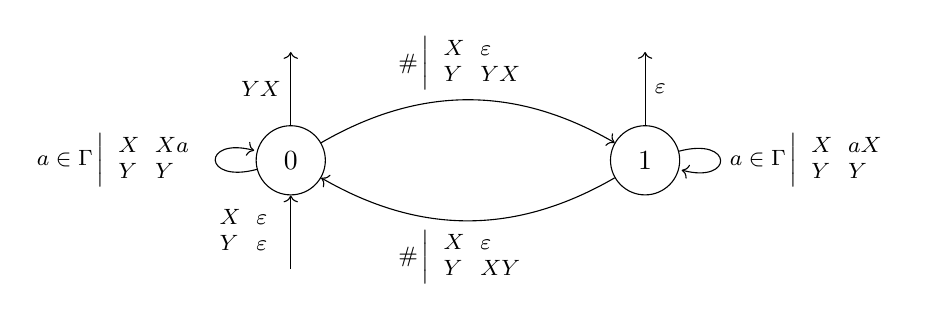
\begin{tikzpicture}[->,node distance=1.5cm]
    %[->,node distance=3.5cm,transform canvas={scale=1}]
    %every text node part/.style={font=\footnotesize}]
    \node[state] (A) {0} ;
    \node (D) [right of=A] {};
    \node (E) [right of=D] {};
    \node[state] (B) [right of=E] {1};
    \node (I) [below of=A] {};
    \node (OA) [above of=A] {};
    \node (OB) [above of=B] {};
  
  \path
    (I) edge node[left, style={font=\footnotesize}]
   {$\begin{array}{l@{~}c@{~}l} X &\regassign& \varepsilon \\ Y &\regassign& \varepsilon \end{array}$} (A) ;
  \path
    (A) edge node[left, style={font=\footnotesize}]
   {$YX$} (OA) ;
  \path
    (B) edge node[right, style={font=\footnotesize}]
   {$\varepsilon$} (OB) ;
  \path
    (A) edge [bend left] node[above, style={font=\footnotesize}]
   {$\#\left| \begin{array}{l@{~}c@{~}l} X &\regassign& \varepsilon \\ Y &\regassign& YX \end{array} \right.$} (B) ;
  \path (B) edge [loop right] node[right,style={font=\footnotesize}]
  {$a \in \Gamma \left| \begin{array}{l@{~}c@{~}l} X &\regassign& aX \\ Y &\regassign& Y \end{array} \right.$}
  (A) ;
  \path (B) edge [bend left] node[below,style={font=\footnotesize}]
   {$\#\left| \begin{array}{l@{~}c@{~}l} X &\regassign& \varepsilon \\ Y &\regassign& XY \end{array} \right.$}
  (A) ;
  \path (A) edge [loop left] node[left,style={font=\footnotesize}]
  {$a \in \Gamma \left| \begin{array}{l@{~}c@{~}l} X &\regassign& Xa \\ Y &\regassign& Y \end{array} \right.$}
  (A) ;
  \end{tikzpicture}
\end{center}
It computes the string-to-string function:
  \[
  \begin{array}{rcl!{\hspace{7em}} l}
  (\Gamma \sqcup \{ {\#} \})^* &\to& \Gamma^*
  & {(w_i \in \Gamma^*,\; (\Gamma \sqcup \{\#\})^* \cong \Gamma^*(\#\Gamma^*)^*)}\\
  w_0\#\ldots\#w_{2k} &\mapsto& \multicolumn{2}{l}{
    \ttreverse(w_{2k-1})
    \ttreverse(w_{2k-3})
    \ldots
    \ttreverse(w_1)
    w_0
    w_2
    \ldots
    w_{2k}} \\
  w_0\#\ldots\#w_{2k+1} &\mapsto& \varepsilon
  \end{array}
  \]
The SST starts out in the initial state $0$, with the initial values of $X$ and $Y$ both set to $\varepsilon$. At each transition, the new values of the registers are computed from the old ones by a parallel assignment. So for example, after reading $aab\#bbc$ (for $a,b,c\in\Gamma$), we are in state $1$ with the register contents $X = cbb$ and $Y = aab$. Finally, if the final state is $0$, the transducer outputs $(\text{final value of}\ Y)\cdot(\text{final value of}\ X)$; if the final state is $1$, it outputs the empty word.
\end{example}

Formally, a \emph{substitution} for the register set $R$ over the alphabet $\Gamma$ is a map $\sigma\colon R \to (\Gamma \cup R)^*$ (assuming that $R \cap \Gamma = \varnothing$). Typically, we have $\sigma(X) = Xa$ and $\sigma(Y) = Y$ for the leftmost register update in the state diagram of \Cref{ex:cecilia}. Substitutions \emph{compose}: define
\[ \sigma \substcomp \tau = (\text{the extension of}\ \sigma\ \text{to a monoid endomorphism of}\ (\Gamma \cup R)^*\ \text{fixing}\ \Gamma) \circ \tau \]
for $\sigma,\tau \colon R \to (\Gamma \cup R)^*$. There is some \enquote{contravariance} going on in this definition: even though we use $f \circ g$ to mean \enquote{apply $g$ then $f$} as usual, the register update specified by $\sigma\substcomp\tau$ corresponds to the update given by $\sigma$ followed by the one given by $\tau$. In other words, if we write $\sigma^\dagger \colon (\Gamma^*)^R \to (\Gamma^*)^R$ for the map between register values specified by $\sigma$ -- so in the above example, $\sigma^\dagger(\rho)(X) = \rho(X)\cdot a$ and $\sigma^\dagger(\rho)(Y) = \rho(Y)$ -- then $(\sigma\substcomp\tau)^\dagger = \tau^\dagger \circ \sigma^\dagger$.

To take into account the finite-state control, we consider the notion of \emph{substransition}: a map $\alpha \colon Q \to Q \times (R \to (\Gamma \cup R))^*$ where $Q$ is a set of states. Substransitions also compose (this is an instance of the wreath product construction):
\[ \text{for}\ q\in Q,\quad (\alpha\substcomp\beta)(q) = (q'',\sigma\substcomp\tau)\ \text{where}\ \alpha(q) = (q',\sigma)\ \text{and}\ \beta(q') = (q'',\tau) \]
\begin{definition}
  We write $\SubsTrans(Q,R,\Gamma)$ for the monoid of all substransitions over the set of states $Q$, the set of registers $R$ and the alphabet $\Gamma$, equipped with $\substcomp$.
\end{definition}
We first introduce \emph{copyful} streaming string transducers, which compute a strict superclass of the regular string functions~\cite{CopyfulSST}. Then we introduce the \emph{bounded-copy} restriction, which brings the computational power down to precisely the regular functions. Syntactically, this is a more permissive discipline than the \enquote{copyless} condition mentioned in the introduction; the equivalence between copyless and bounded-copy SSTs was established in\footnote{\tito{Finite coyping~\cite{MacroMSO} = bounded-copy~\cite{AlurFT12} (TODO: check)}
}~\cite[Section~IV.A]{AlurFT12}.

\begin{definition}
  \label{def:sst}
  A (deterministic copyful) \emph{streaming string transducer (SST)} with input
  alphabet $\Sigma$ and output alphabet $\Gamma$ is a tuple $\mathcal{T} = (Q, q_0, R,
  \delta, \vec{u}_I, F)$ where
\begin{itemize}
\item $Q$ is a finite set of \emph{states} and $q_0 \in Q$ is the \emph{initial
    state};
\item $R$ is a finite set of \emph{register names}, that we require to be
  disjoint from $\Gamma$;
\item $\delta \colon \Sigma \to \SubsTrans(Q,R,\Gamma)$ is the \emph{transition function};
\item $\vec{u}_I \in (\Sigma^*)^R$ describes the \emph{initial register values};
\item $F \colon Q \to (\Gamma \cup R)^*$ is the \emph{final output function}.
\end{itemize}
For an input word $w \in \Sigma^*$, the output of $\mathcal{T}$ is determined as follows. Let $(q,\sigma) = \delta^*(w)(q_0)$ where $\delta^*$ is the unique extension of $\delta$ to a monoid homomorphism $\Sigma^* \to \SubsTrans(Q,R,\Gamma)$. Apply $\sigma^\dagger \colon (\Gamma^*)^R \to (\Gamma^*)^R$ to $\vec{u}_I$ to get a tuple $\vec{v} = (v_X)_{X\in R}$ of final register values. Finally, replace each occurrence in $F(q)$ of a register name $X\in R$ by the corresponding value $v_X \in \Gamma^*$ to obtain an output string in $\Gamma^*$.
\end{definition}
\begin{definition}[see e.g.~{\cite{AlurFT12,AperiodicSST}}]
  A streaming string transducer whose transition function is $\delta \colon \Sigma \to \SubsTrans(Q,R,\Gamma)$ is \emph{bounded-copy} when there is some bound $k\in\mathbb{N}$ such that for every $q\in Q$, $w \in \Gamma^*$ and $X,Y\in R$, the string $\sigma(X)$ where $\delta^*(w)(q) = (q',\sigma)$ contains at most $k$ occurrences of~$Y$.
  In this paper, we take computability by bounded-copy SSTs as the definition of \emph{regular string-to-string functions}.
\end{definition}
The SST of \Cref{ex:cecilia} is bounded-copy (see \Cref{ex:cecilia-monoid} below). The following example of streaming string transducer is \emph{not} bounded-copy: it has a single state $q$ and a single register $X$; it performs $X \regassign XX$ for each input letter; the initial value is $X = a$ and the final output function is $F(q) = X$. This SST computes the function is $w \mapsto a\dots(2^{|w|}\ \text{times})\dots a$ which is not a regular function since its growth is not linearly bounded. Observe that the substitution $\sigma$ corresponding to an input factor $w$ is $\sigma \colon X \mapsto X\dots(2^{|w|}\ \text{times})\dots X$ -- this violates the bounded-copy condition.

The notion of bounded-copy SST can be rephrased using the monoid homomorphism $\tterase_\Gamma \colon \SubsTrans(Q,R,\Gamma) \to \SubsTrans(Q,R,\varnothing)$ which \enquote{erases all letters from $\Gamma$}, built by lifting the homomorphism $w \in \Gamma^* \mapsto \varepsilon \in \varnothing^*$ in the unique sensible way. 
\begin{proposition}\label{prop:bounded-copy-finiteness}
  An SST with transition function $\delta \colon \Sigma \to \SubsTrans(Q,R,\Gamma)$ is bounded-copy if and only if $\tterase_\Gamma(\delta^*(\Sigma^*))$ is a \emph{finite} submonoid of $\SubsTrans(Q,R,\varnothing)$. 
\end{proposition}
\begin{remark}
  This monoid $\tterase_\Gamma(\delta^*(\Sigma^*))$ is called the \emph{substitution transition monoid} of the given SST in~\cite[Section~3]{AperiodicSST}.
\end{remark}
\begin{example}\label{ex:cecilia-monoid}
  For the streaming string transducer of \Cref{ex:cecilia} (recall that its input alphabet is $\Gamma\cup\{\#\}$), we have (abbreviating $\ttreverse(w)$ by $\widetilde{w}$):
  \begin{align*}
    \text{for}\ w\in\Gamma^*,\; \delta^*(w) &= \begin{cases}
      0 \mapsto (0, (X \mapsto Xw \mid Y \mapsto Y))\\
      1 \mapsto (1, (X \mapsto \widetilde{w}X \mid Y \mapsto Y))
    \end{cases}\\
    \delta^*(w_0 \# \dots \# w_{2k+1}) &= \begin{cases}
      0 \mapsto (1, (X \mapsto \widetilde{w_{2k+1}} \mid Y \mapsto \widetilde{w_{2k-1}} \dots \widetilde{w_1} YX w_0 \dots w_{2k}))\\
      1 \mapsto (0, (X \mapsto w_{2k+1} \mid Y \mapsto \widetilde{w_{2k}} \dots \widetilde{w_0}XY w_1 \dots w_{2k-1}))
    \end{cases}\\
    \delta^*(w_0 \# \dots \# w_{2k+2}) &= \begin{cases}
      0 \mapsto (0, (X \mapsto w_{2k+2} \mid Y \mapsto \widetilde{w_{2k+1}} \dots \widetilde{w_1}YX w_0 \dots w_{2k}))\\
      1 \mapsto (1, (X \mapsto \widetilde{w_{2k+2}} \mid Y \mapsto \widetilde{w_{2k}} \dots \widetilde{w_0} XY w_1 \dots w_{2k+1}))
    \end{cases}
  \end{align*}
  By erasing the parts in $\Gamma^*$ of the right-hand sides, we see that the substitution transition monoid has three elements: the identity (which is the image of all words without $\#$) and
  \[ \begin{cases}
    0 \mapsto (1, (X \mapsto \varepsilon \mid Y \mapsto YX))\\
    1 \mapsto (0, (X \mapsto \varepsilon \mid Y \mapsto XY))
  \end{cases} \qquad\quad \begin{cases}
    0 \mapsto (0, (X \mapsto \varepsilon \mid Y \mapsto YX))\\
    1 \mapsto (1, (X \mapsto \varepsilon \mid Y \mapsto XY))
  \end{cases} \]
  Hence, since $3 < \infty$, the SST of \Cref{ex:cecilia} is bounded-copy.
\end{example}


\section{Register transducer semigroups}

We now introduce our first definition of regular semigroup-to-semigroup functions, heavily inspired by streaming string transducers. In the definition below, the maps $\mu_{s_1,s_2}$ should be understood as analogous to the substitutions in SSTs. At the same time, the whole definition itself can be seen at first as an abstraction of the monoid denoted by $\delta^*(\Sigma^*)$ in the previous section -- though we will see that even for string-to-string functions, we have good reasons to work with semigroups rather than monoids.

\begin{definition}
    A \emph{finitary semigroup with registers} $\mathcal{S}$ consists of a finite semigroup $S$, a family $(R_s)_{s\in S}$ of finite nonempty sets, and a family of functions
    \[ \mu_{s_1, s_2}\colon R_{s_1 s_2} \to (R_{s_1} + R_{s_2})^+ \quad\text{for}\ s_1, s_2 \in S\]
    such that for all $s_1, s_2, s_3 \in S$, the following associativity diagram
    commutes:
    \[\begin{tikzcd}
        [column sep=2.5cm]
        &
        (R_{s_1 s_2} + R_{s_3})^+
        \ar[r,"(\mu_{s_1,s_2}+\mathrm{id})^+"']
        &
        ((R_{s_1}+R_{s_2})+R_{s_3})^+
        \ar[dd,"\text{assoc.\ of}\ +"]
        \\
        R_{s_1 s_2 s_3}
        \ar[ur,"\mu_{s_1s_2,s_3}"]
        \ar[dr,"\mu_{s_1,s_2s_3}"']
        \\
        &
        (R_{s_1} + R_{s_2 s_3})^+
        \ar[r,"(\mathrm{id}+\mu_{s_2,s_3})^+"]
        &
        (R_{s_1}+(R_{s_2}+R_{s_3}))^+
      \end{tikzcd}\]
    For any semigroup $A$, we define $\mathcal{S}[A] = \displaystyle\bigcup_{s\in S} \{s\} \times A^{R_s}$
    endowed with the binary operation
    \[ (s_1,(a_{1,X})_{X\in R_{s_1}}) \cdot (s_2,(a_{2,Y})_{Y\in R_{s_2}}) = (s_1 s_2,\, (\overbrace{\mathrm{flatten}}^{\mathclap{A^+ \to A\ \text{using the semigroup operation in}\ A}} \circ \underbrace{\mathrm{substitute}}_{\mathclap{\text{replace each}\ X \in R_{s_1}\ \text{(resp.\ $Y \in R_{s_2}$) by}\ a_{1,X}\ \text{(resp.\ $a_{2,Y}$)}}} \circ \mu_{s_1 s_2}(Z))_{Z\in R_{s_1 s_2}}) \]
\end{definition}
\begin{proposition}
  For any finitary semigroup with registers $\mathcal{S}$ and any semigroup $A$, the binary operation on $\mathcal{S}[A]$ is associative: $\mathcal{S}[A]$ is a semigroup.
\end{proposition}
\begin{example}\label{ex:fsr-simple}
  Let $S = \{0,1\}$ with usual multiplication and $R_0 = R_1 = \{X,Y\}$. Let us write $\{X,Y\}+\{X,Y\}=\{X_{\mathrm{l}}, X_{\mathrm{r}}, Y_{\mathrm{l}}, Y_{\mathrm{r}}\}$ with $X_{\mathrm{l}}$ (resp.~$X_{\mathrm{r}}$) referring to the left (resp.~right) copy of $X$. The following definition of $\mu$ satisfies the associativity condition:
  \[ \forall i,j \in \{0,1\}, \qquad \mu_{i,j}(X) = X_{\mathrm{l}} X_{\mathrm{r}} \qquad \mu_{i,0}(Y) = X_{\mathrm{l}} Y_{\mathrm{r}} \qquad \mu_{i,1}(Y) = Y_{\mathrm{l}} Y_{\mathrm{r}} \]
  So $\mathcal{S} = (S,R,\mu)$ is a finitary semigroup with registers. We have for example in $\mathcal{S}[(\mathbb{N},+)]$
  \[ (1,(X\mapsto42\mid Y\mapsto218)) \cdot (0,(X\mapsto1\mid Y\mapsto100)) = (0,(X\mapsto43\mid Y\mapsto142)) \]
\end{example}

\begin{definition}\label{def:reg-trans-semigroup}
    A \emph{register transducer semigroup} consists of a finitary semigroup with registers $\mathcal{S} = (S,R,\mu)$ together with a family of strings $\omega_s \in (R_s)^+$ for $s\in S$.

    A function $f\colon A \to B$ between semigroups is said to be \emph{recognized} by $(\mathcal{S}, \omega)$ if it admits a decomposition $f = \outfun_B \circ h$ where $h \colon A \to \mathcal{S}[B]$ is some semigroup homomorphism and
    \[ \outfun_B(s,(b_X)_{X \in R_s}) = \mathrm{flatten}(\text{replace each}\ X\in R_s\ \text{in}\ \omega_s\ \text{by}\ b_X) \]
    $f$ is called \emph{regular} when there exists a register transducer semigroup that recognizes it.
\end{definition}
\begin{example}\label{ex:rts-simple}
  Let $\mathcal{S}$ be the finitary semigroup with registers from \Cref{ex:fsr-simple}. Reusing the notations from that example, let us choose $\omega_0 = \omega_1 = Y$; this makes $(\mathcal{S},\omega)$ is a register transducer semigroup. It can recognize the function $f\colon \{a,b,c\}^* \to \{a,b\}^*$ such that
  \[ \forall u \in \{a,b,c\}^*,\;\forall v \in \{a,b\}^*,\quad f(ucv) = a^{|u|}bv \quad\text{and}\quad f(v) = v \]
  (inspired by~\cite[Theorem~5.6]{MacroMSO}). Indeed, to do so, we pick the semigroup homomorphism
  \[ h\colon w \in \{a,b,c\}^* \mapsto ((1\ \text{if}\ w\in\{a,b\}^*,\;\text{else}\ 0),\; (X\mapsto a^{|w|} \mid Y \mapsto f(w)) \in \mathcal{S}[\{a,b\}^*]\]
\end{example}

\begin{theorem}
  A function between free monoids is regular in the sense of \Cref{def:reg-trans-semigroup} (i.e.\ recognized by some register transducer semigroup) if and only if it is a regular string function in the conventional sense (i.e.\ computed by some bounded-copy SST).
\end{theorem}
\begin{proof}
  We first treat \enquote{only if}, then \enquote{if}.

  \proofsubparagraph{From a register transducer semigroup to a bounded-copy streaming string transducer.}
  Let $(\mathcal{S}=(S,R,\mu),\,\omega)$ be a register transducer semigroup and $h\colon \Sigma^* \to \mathcal{S}[\Gamma^*]$ be a semigroup homomorphism. We want a bounded-copy SST that computes $\outfun_{\Gamma^*}\circ h$. Our solution will be to take an \enquote{obvious choice} of SST, which clearly computes this function -- the idea is that the configuration (state + register contents) of the SST, after reading an input prefix $w\in\Sigma^*$, represents $h(w)$ -- and then check that it is bounded-copy.
  \begin{itemize}
    \item The set of states is $Q = S$ and the initial state is the first component of $h(\varepsilon)$. (Note that while $\mathcal{S}[\Gamma^*]$ is not necessarily a monoid, $h(\Sigma^*)$ always is, with $h(\varepsilon)$ as its unit element.)
    \item The registers are $R = \displaystyle\bigcup_{s\in S} R_s$ (without loss of generality, we take the $R_s$ pairwise disjoint).
    \item For $c\in\Sigma$ and $q\in Q=S$, we define $\delta(c)(q) = (qs,\sigma)$ where $(s, (v_X)_{X\in R_s}) = h(c)$ and
    \[ \sigma\colon Y \in R ~~\mapsto~~ \begin{cases}
      \text{replace each}\ X \in R_s\ \text{by}\ v_X\ \text{in}\ \mu_{q,s}(Y) & \text{when}\ Y \in R_{qs}\\
      \varepsilon & \text{otherwise}
    \end{cases} \]
    \item The initial register values are $X:=u_{0,X}$ for any $X\in R_{q_0}$ where $(q_0,(u_{0,X})_{X\in R_{q_0}}) = h(\varepsilon)$, and $X := \varepsilon$ for other registers.
    \item The final output function is $q \mapsto \omega_q$.
  \end{itemize}
  One can verify that $\tterase_\Gamma(\delta^*(w))(q) = (qs, [\text{something fully determined by}\ \mu_{q,s}])$ where $s$ is the 1st component of $h(w)$ for any $w\in\Sigma^*$ and $q\in Q$. Since $s$ lives in the finite semigroup~$S$, the monoid $\tterase_\Gamma(\delta^*(\Sigma^*))$ is finite. By \Cref{prop:bounded-copy-finiteness}, our SST is bounded-copy.

  \proofsubparagraph{From a bounded-copy streaming string transducer to a register transducer semigroup.}

  We start by illustrating the main idea on the SST of \Cref{ex:cecilia}. This SST has several convenient properties that simplify the construction (in particular, the semigroup that we get is a monoid): all its registers are initialized with $\varepsilon$, and the final output function merely combines registers without adding letters from the output alphabet. We will see later how to handle the minor complications that may arise without these properties.
  \begin{claim}
    The function $\Sigma^* \to \Gamma^*$ (with $\Sigma = \Gamma\cup\{\#\}$) of \Cref{ex:cecilia} is recognized by a register transducer semigroup $(\mathcal{M} = (M,R,\mu),\; \omega)$, where $M = \tterase_\Gamma(\delta^*(\Sigma^*))$ is the finite substitution transition monoid described in \Cref{ex:cecilia-monoid}, and such that the infinite monoid $\delta^*(\Sigma^*)$ can be identified with a submonoid of $\mathcal{M}[\Gamma^*]$.
  \end{claim}
  \begin{claimproof}[Proof sketch]
    We shall work with the following abbreviations for $u,v,\ldots \in \Sigma^*$:
    \begin{align*}
      \alpha[u,v] &= \begin{cases}
        0 \mapsto (0, (X \mapsto Xu \mid Y \mapsto Y))\\
        1 \mapsto (1, (X \mapsto vX \mid Y \mapsto Y))
      \end{cases}\\
      \text{for}\ i \in \{0,1\},\quad \beta_i[u_1,\dots,v_3] &= \begin{cases}
        0 \mapsto (i,\quad\;\; (X \mapsto u_1 \mid Y \mapsto u_2 YX u_3))\\
        1 \mapsto (1-i, (X \mapsto v_1 \mid Y \mapsto v_2 XY v_3))
      \end{cases}      
    \end{align*}
    We also write $\alpha = \alpha[\varepsilon,\varepsilon]$ and $\beta_i = \beta_i[\varepsilon,\dots,\varepsilon]$.
    Note that $M = \{\alpha,\beta_0,\beta_1\}$ (equipped with composition of substransitions), while every element of $\delta^*(\Sigma^*)$ is of the form $\alpha[\dots]$ or $\beta_i[\dots]$. The set $\mathfrak{M}$ of all $\alpha[\dots]$ and $\beta_i[\dots]$ is a submonoid of $\SubsTrans(\{0,1\},\{X,Y\},\Gamma)$, since $\alpha$ is the unit element and we have composition equations such as
    \[ \alpha[u,v] \cdot \beta_1[u_1,\dots,v_3] = \beta_1[u_1,u_2,(u \cdot u_3),v_1,(v_2 \cdot v),v_3] \]
    The idea is then to define $\mathcal{M} = (M,R,\mu)$ in such a way that $\mathfrak{M} \cong \mathcal{M}[\Gamma^*]$. We take $R_\alpha = \{1,2\}$ and $R_{\beta_i} = \{1,2\} \times \{1,2,3\}$. This allows us to define a bijection
    \begin{align*}
      \mathcal{M}[\Gamma^*] &\to \mathfrak{M}\\
      (\alpha, (w_1, w_2)) &\mapsto \alpha[w_1,w_2]\\
      (\beta_i, (w_{1,1},\dots,w_{2,3})) &\mapsto \beta_i[w_{1,1},\dots,w_{2,3}]
    \end{align*}
    Observe also that for $\lambda,\gamma\in\{\alpha,\beta_0,\beta_1\}$, we have $\lambda[\dots] \cdot \gamma[\dots] = (\lambda\cdot\gamma)[\dots]$, which brings us halfway to having the above bijection be a monoid isomorphism. To get there, there remains to choose a definition of $\mu$ reflecting the composition equations; for example the above one concerning $\alpha$ and $\beta_1$ leads us to define $\mu_{\alpha,\beta_1}$ as
    \[ (1,1)\mapsto(1,1) \mid \dots \mid (1,3) \mapsto 1 \cdot (1,3) \mid \dots \mid (2,2) \mapsto (2,2) \cdot 2 \mid (2,3) \mapsto (2,3) \]
    We set the output strings of our register transducer semigroup according to the initial state and final output function of \Cref{ex:cecilia}, as follows:
    \begin{itemize}
      \item $\omega_\alpha = 1$ because after applying $\alpha[u,v]$ to the initial configuration of the SST, we are in state 0, $X = u$ \& $Y = \varepsilon$, and the final output function tells us to output $YX = u$;
      \item $\omega_{\beta_0} = (1,2)\cdot(1,3)\cdot(1,1)$ because after applying $\beta_0[u_1,\dots,v_3]$ to the initial configuration, we are in state 0 and $X$ contains $u_1$ while $Y$ contains $u_2 u_3$;
      \item $\omega_{\beta_1} = \varepsilon$ because applying $\beta_1[\dots]$ to the initial configuration brings us in state 1, in which the final output function tells us to output $\varepsilon$.
    \end{itemize}
    Finally, to recognize the function of \Cref{ex:cecilia}, we use the semigroup homomorphism $(\text{inverse of above isomorphism}\ \mathcal{M}[\Gamma^*] \to \mathfrak{M}) \circ \delta^* : \Sigma^* \to \mathcal{M}[\Gamma^*]$.
  \end{claimproof}

  \tito{todo}
\end{proof}

\tito{Probably in the final paper it would be nice to introduce these things without invoking categories at first, to make the paper more welcoming}


\begin{remark}
  This data induces the finite polynomial functor from semigroups to sets BLAH  
  which can be turned into a functor from semigroups to semigroups thanks to $\mu$.


    Equivalently, consider the following symmetric monoidal category:
    \begin{description}
        \item[Objects:] finite polynomial functors (in one variable).
        \item[Morphisms:] natural transformations.
        \item[Monoidal product:] pointwise cartesian product of sets.
    \end{description}
    A finitary semigroup with registers is the same thing as a \enquote{semigroup object} (defined by removing the unit requirement from monoid objects) in this monoidal category of finite polynomial functors.

    \tito{Blah is equivalent to specifying a natural transformation from the associated polynomial functor to the forgetful functor from semigroups to sets, so it induces a functorial transducer semigroup in the expected way.}
\end{remark}


\begin{remark}
This should also work if we have a single finite nonempty set of registers $R$ for all semigroup elements instead of a family $(R_s)_{s\in S}$ though the equivalence proof is slightly less immediate for semigroups than for monoids (you need to use the output function to produce \enquote{default} elements with which to fill unused registers). Note that the \enquote{substitution transition monoid} operation \enquote{naturally} produces something with a varying register set.

Another possible variation on the definition is to have a choice of output register for each element of the control semigroup: $r_s \in R_s$ for $s\in S$ instead of $\omega_s \in (R_s)^+$. This does not decrease the expressivity of the model.
\end{remark}



\section{Equivalence with functorial transducer semigroups}

It is immediate that every regular function is recognized by a finiteness-preserving functorial transducer semigroup, because finite polynomial functors are finiteness-preserving. We shall therefore focus on the converse.

\begin{theorem}
  For every finiteness-preserving functorial transducer semigroup $(\functor, \outfun)$, there is another one $(\functor',\outfun')$
  \begin{itemize}
    \item which is induced by some register transducer semigroup,
    \item and which admits a natural transformation $\eta \colon \functor \Rightarrow \functor'$ such that $\outfun = \outfun' \circ \eta$.
  \end{itemize}
  Hence every function recognized by $(\functor,\outfun)$ is also recognized by $(\functor',\outfun')$ (by the second item) and thus is regular (by the first item).
\end{theorem}
\begin{proof}
    Let $(\functor,\outfun)$ be a functorial transducer semigroup, and suppose $\functor$ preserves finiteness, so $\functor1$ is finite. We first build a finitary semigroup with registers that doesn't entirely fulfill our objectives, but still contains the core mechanism: $S = \functor1$, and for $s\in S$,
    \[ R_s = \sum_{l,r \in F(1)} \{\text{occurrences of}\ \mathtt{m}\ \text{in}\ (\text{factorized output of}\ (l,s,r)) \in 1\oplus1\oplus1 \cong \{\mathtt{l,m,r}\}^+\} \]
    For $s_1,s_2\in S$ we must now define a map $R_{s_1 s_2} \to (R_{s_1} + R_{s_2})^+$ describing the register recombination during a product. We derive it from the correspondence between
    \begin{itemize}
        \item the occurrences of $\mathtt{m}$ in the factorized output of $l \cdot (s_1 s_2)\cdot r$
        \item and the maximal factors in $\{\mathtt{m_1,m_2}\}^+$ inside
        \[ (\text{factorized output of}\ (l,s_1,s_2,r)) \in 1\oplus1\oplus1\oplus1 \cong \{\mathtt{l,m_1,m_2,r}\}^+ \]
    \end{itemize}
    Indeed, the morphism $1\oplus\mathop{!}\oplus1$ where $! \colon 1\oplus1 \to 1$ is the terminal morphism sends the maximal factors in $\{\mathtt{m_1,m_2}\}^+$ to $\mathtt{m}$ and is the identity on $\mathtt{l,r}$. To see that applying this to the factorized output of $(l,s_1,s_2,r)$ indeed yields the factorized output of $(l,s_1s_2,r)$, apply \Cref{lem:merge-middle} to $A=B=C=1$.

    We must also check that this operation is \enquote{associative}. For this, consider the factorized output of $(l,s_1,s_2,s_3,r)$ \ldots{}
    \tito{TODO above}

    Finally we define $\widehat\eta \colon \functor \Rightarrow \functorg$ where $\functorg$ is the functor induced by our semigroup with registers. For any $x \in \functor A$, apply $\functor! \colon \functor A \to \functor 1$ to get some $s \in S$. Then look at the factorized output of $(l,x,r)$ in $1\oplus A \oplus 1$ for each $(l,r)\in (\functor1)^2$ to get register values in $A^{R_s}$.

    The issue is that the output function for $\functor$ may not factor through $\widehat\eta$. To remediate that, we consider instead another semigroup with registers, inducing the functor $\functor'$, with the same underlying semigroup $S=\functor1$ and bigger register sets
    \[ R'_s = \{\bullet\} + R^{\mathrm{left}}_s + R^{\mathrm{right}}_s + R_s \quad\text{for}\ s\in S\]
    where $R^{\mathrm{left}}_s$ is the sum over $r \in \functor1$ of the sets of occurrences of $\mathtt{l}$ in the factorized output of $(s,r)$ which is in $1\oplus1\cong\{\mathtt{l,r}\}^+$, etc. Thus
    \[ \functor'A \cong \sum_{s\in S} A \times A^{R^{\mathrm{left}}_s} \times \dots \cong A \times \sum_{s\in S} A^{R^{\mathrm{left}}_s} \times \dots \]
    and we have then: $\outfun_A = (\text{left projection on}\ A) \circ \eta$ for the definition of $\eta$ extending $\widehat\eta$ in the obvious way.
\end{proof}

\begin{lemma}\label{lem:merge-middle}
    Let $A,B,C$ be semigroups. The following diagram commutes:
    \[\begin{tikzcd}
        [column sep=3cm]
        \functor A \times \functor B\times \functor B \times \functor C
        \ar[r,"\text{factorized output}"]
        \ar[d,"\functor A \times (\text{semigroup operation}) \times \functor C"']
        &
        A \oplus B \oplus B \oplus C
        \ar[d,"A \oplus (\mathrm{id}_B\,\text{or}\,\mathrm{id}_B) \oplus C"]
        \\
        \functor A \times \functor B \times \functor C
        \ar[r,"\text{factorized output}"]
        &
        A \oplus B \oplus C
    \end{tikzcd}\]
\end{lemma}
\tito{similar to \Cref{claim:merge-factorized-output}}
\begin{proof}
    By rotating the above diagram, we see that it corresponds to the outer rectangle in the following diagram (where we have expanded the definition of the factorized output functions, and used the associativity of 4-fold multiplication):
    \[\begin{tikzcd}
        [column sep=4cm]
        \functor A \times \functor B\times \functor B \times \functor C
        \ar[d,"\functor(\text{co-projection})^4"']
        \ar[r,"\functor A \times (\text{semigroup op}) \times \functor C"]
        &
        \functor A \times \functor B \times \functor C
        \ar[d,"\functor(\text{co-projection})^3"]
        \\
        \functor(A \oplus B \oplus B \oplus C)^4
        \ar[d,"\text{multiply middle two together}"']
        &
        \functor(A \oplus B \oplus C)^3
        \ar[dd,""]
        \\
        \functor(A \oplus B \oplus B \oplus C)^3
        \ar[d,"\text{semigroup operation}"']
        \ar[ru,"F(A \oplus (\mathrm{id}_B\,\text{or}\,\mathrm{id}_B) \oplus C)^3"']
        \\
        \functor(A \oplus B \oplus B \oplus C)
        \ar[d, "\outfun_{A \oplus B \oplus B \oplus C}"']
        \ar[r,"F(A \oplus (\mathrm{id}_B\,\text{or}\,\mathrm{id}_B) \oplus C)"]
        &
        \functor(A \oplus B \oplus C)
        \ar[d, ""]
        \\ 
        A \oplus B \oplus B \oplus C
        \ar[r,"A \oplus (\mathrm{id}_B\,\text{or}\,\mathrm{id}_B) \oplus C"]
        &
        A \oplus B \oplus C
    \end{tikzcd}\]
    The lower rectangle commutes by naturality of the output function. The middle trapeze commutes because of the homomorphism property of $F(A \oplus (\mathrm{id}_B\,\text{or}\,\mathrm{id}_B) \oplus C)$. Concerning the upper trapeze, it can be decomposed as the functor $(\cdots \times \cdots \times \cdots)$ applied to three diagrams that we can analyze independently. The first of those is
    \[\begin{tikzcd}
        [column sep=4cm]
        \functor A
        \ar[d,"\functor(\text{co-projection})"']
        \ar[r,"\mathrm{id}_A"]
        &
        \functor A
        \ar[d,"\functor(\text{co-projection})"]
        \\
        \functor(A \oplus B \oplus B \oplus C)
        \ar[d,"\mathrm{id}"']
        &
        \functor(A \oplus B \oplus C)
        \\
        \functor(A \oplus B \oplus B \oplus C)
            \ar[ru,"F(A \oplus (\mathrm{id}_B\,\text{or}\,\mathrm{id}_B) \oplus C)"']
    \end{tikzcd}\]
    By functoriality of $\functor$, the commutativity of this diagram reduces to
    \[ (\mathrm{id}_A \oplus \dots) \circ (\text{co-projection of}\ A\ \text{into}\ A\oplus(B\oplus B\oplus C)) = \text{co-projection of}\ A\ \text{into}\ A\oplus(B\oplus C) \]
    which is an elementary property of the coproduct $\oplus$ in any category (indeed the bifunctor structure of $\oplus$ is built using a coparing, which \enquote{cancels out} with the coprojection).
    Among the 3 diagrams that were combined by a 3-fold cartesian product, another one is identical to the above, with $C$ replacing $A$. There remains this one, in which we have added some parts in the middle:
    \[\begin{tikzcd}
        [column sep=2.5cm]
        \functor B\times \functor B
        \ar[d,"\functor(\text{co-proj})^2"']
        \ar[dr,"\functor(\text{co-proj})^2"]
        \ar[rr,"\text{semigroup operation}"]
        &
        &
        \functor B
        \ar[d,"\functor(\text{co-proj})"]
        \\
        \functor(A \oplus B \oplus B \oplus C)^2
        \ar[d,"\text{semigroup op}"']
        \ar[r,"h\times h"']
        &
        \functor(A \oplus B \oplus C)^2
        \ar[r,"\text{semigroup op}"]
        &
        \functor(A \oplus B \oplus C)
        \\
        \functor(A \oplus B \oplus B \oplus C)
            \ar[rru,"h = F(A \oplus (\mathrm{id}_B\,\text{or}\,\mathrm{id}_B) \oplus C)"']
    \end{tikzcd}\]
    The upper right trapeze commutes because $\functor$ applied to the co-projection of $B$ into $A\oplus B\oplus C$ is a homomorphism. The lower triangle commutes because $h$ is a homomorphism. Finally, the small upper left triangle can be shown to commute using the functoriality of $\functor$ followed by properties of the coproduct.
\end{proof}


\end{document}
